
% Default to the notebook output style

    


% Inherit from the specified cell style.




    
\documentclass[11pt]{article}

    
    
    \usepackage[T1]{fontenc}
    % Nicer default font (+ math font) than Computer Modern for most use cases
    \usepackage{mathpazo}

    % Basic figure setup, for now with no caption control since it's done
    % automatically by Pandoc (which extracts ![](path) syntax from Markdown).
    \usepackage{graphicx}
    % We will generate all images so they have a width \maxwidth. This means
    % that they will get their normal width if they fit onto the page, but
    % are scaled down if they would overflow the margins.
    \makeatletter
    \def\maxwidth{\ifdim\Gin@nat@width>\linewidth\linewidth
    \else\Gin@nat@width\fi}
    \makeatother
    \let\Oldincludegraphics\includegraphics
    % Set max figure width to be 80% of text width, for now hardcoded.
    \renewcommand{\includegraphics}[1]{\Oldincludegraphics[width=.8\maxwidth]{#1}}
    % Ensure that by default, figures have no caption (until we provide a
    % proper Figure object with a Caption API and a way to capture that
    % in the conversion process - todo).
    \usepackage{caption}
    \DeclareCaptionLabelFormat{nolabel}{}
    \captionsetup{labelformat=nolabel}

    \usepackage{adjustbox} % Used to constrain images to a maximum size 
    \usepackage{xcolor} % Allow colors to be defined
    \usepackage{enumerate} % Needed for markdown enumerations to work
    \usepackage{geometry} % Used to adjust the document margins
    \usepackage{amsmath} % Equations
    \usepackage{amssymb} % Equations
    \usepackage{textcomp} % defines textquotesingle
    % Hack from http://tex.stackexchange.com/a/47451/13684:
    \AtBeginDocument{%
        \def\PYZsq{\textquotesingle}% Upright quotes in Pygmentized code
    }
    \usepackage{upquote} % Upright quotes for verbatim code
    \usepackage{eurosym} % defines \euro
    \usepackage[mathletters]{ucs} % Extended unicode (utf-8) support
    \usepackage[utf8x]{inputenc} % Allow utf-8 characters in the tex document
    \usepackage{fancyvrb} % verbatim replacement that allows latex
    \usepackage{grffile} % extends the file name processing of package graphics 
                         % to support a larger range 
    % The hyperref package gives us a pdf with properly built
    % internal navigation ('pdf bookmarks' for the table of contents,
    % internal cross-reference links, web links for URLs, etc.)
    \usepackage{hyperref}
    \usepackage{longtable} % longtable support required by pandoc >1.10
    \usepackage{booktabs}  % table support for pandoc > 1.12.2
    \usepackage[inline]{enumitem} % IRkernel/repr support (it uses the enumerate* environment)
    \usepackage[normalem]{ulem} % ulem is needed to support strikethroughs (\sout)
                                % normalem makes italics be italics, not underlines
    

    
    
    % Colors for the hyperref package
    \definecolor{urlcolor}{rgb}{0,.145,.698}
    \definecolor{linkcolor}{rgb}{.71,0.21,0.01}
    \definecolor{citecolor}{rgb}{.12,.54,.11}

    % ANSI colors
    \definecolor{ansi-black}{HTML}{3E424D}
    \definecolor{ansi-black-intense}{HTML}{282C36}
    \definecolor{ansi-red}{HTML}{E75C58}
    \definecolor{ansi-red-intense}{HTML}{B22B31}
    \definecolor{ansi-green}{HTML}{00A250}
    \definecolor{ansi-green-intense}{HTML}{007427}
    \definecolor{ansi-yellow}{HTML}{DDB62B}
    \definecolor{ansi-yellow-intense}{HTML}{B27D12}
    \definecolor{ansi-blue}{HTML}{208FFB}
    \definecolor{ansi-blue-intense}{HTML}{0065CA}
    \definecolor{ansi-magenta}{HTML}{D160C4}
    \definecolor{ansi-magenta-intense}{HTML}{A03196}
    \definecolor{ansi-cyan}{HTML}{60C6C8}
    \definecolor{ansi-cyan-intense}{HTML}{258F8F}
    \definecolor{ansi-white}{HTML}{C5C1B4}
    \definecolor{ansi-white-intense}{HTML}{A1A6B2}

    % commands and environments needed by pandoc snippets
    % extracted from the output of `pandoc -s`
    \providecommand{\tightlist}{%
      \setlength{\itemsep}{0pt}\setlength{\parskip}{0pt}}
    \DefineVerbatimEnvironment{Highlighting}{Verbatim}{commandchars=\\\{\}}
    % Add ',fontsize=\small' for more characters per line
    \newenvironment{Shaded}{}{}
    \newcommand{\KeywordTok}[1]{\textcolor[rgb]{0.00,0.44,0.13}{\textbf{{#1}}}}
    \newcommand{\DataTypeTok}[1]{\textcolor[rgb]{0.56,0.13,0.00}{{#1}}}
    \newcommand{\DecValTok}[1]{\textcolor[rgb]{0.25,0.63,0.44}{{#1}}}
    \newcommand{\BaseNTok}[1]{\textcolor[rgb]{0.25,0.63,0.44}{{#1}}}
    \newcommand{\FloatTok}[1]{\textcolor[rgb]{0.25,0.63,0.44}{{#1}}}
    \newcommand{\CharTok}[1]{\textcolor[rgb]{0.25,0.44,0.63}{{#1}}}
    \newcommand{\StringTok}[1]{\textcolor[rgb]{0.25,0.44,0.63}{{#1}}}
    \newcommand{\CommentTok}[1]{\textcolor[rgb]{0.38,0.63,0.69}{\textit{{#1}}}}
    \newcommand{\OtherTok}[1]{\textcolor[rgb]{0.00,0.44,0.13}{{#1}}}
    \newcommand{\AlertTok}[1]{\textcolor[rgb]{1.00,0.00,0.00}{\textbf{{#1}}}}
    \newcommand{\FunctionTok}[1]{\textcolor[rgb]{0.02,0.16,0.49}{{#1}}}
    \newcommand{\RegionMarkerTok}[1]{{#1}}
    \newcommand{\ErrorTok}[1]{\textcolor[rgb]{1.00,0.00,0.00}{\textbf{{#1}}}}
    \newcommand{\NormalTok}[1]{{#1}}
    
    % Additional commands for more recent versions of Pandoc
    \newcommand{\ConstantTok}[1]{\textcolor[rgb]{0.53,0.00,0.00}{{#1}}}
    \newcommand{\SpecialCharTok}[1]{\textcolor[rgb]{0.25,0.44,0.63}{{#1}}}
    \newcommand{\VerbatimStringTok}[1]{\textcolor[rgb]{0.25,0.44,0.63}{{#1}}}
    \newcommand{\SpecialStringTok}[1]{\textcolor[rgb]{0.73,0.40,0.53}{{#1}}}
    \newcommand{\ImportTok}[1]{{#1}}
    \newcommand{\DocumentationTok}[1]{\textcolor[rgb]{0.73,0.13,0.13}{\textit{{#1}}}}
    \newcommand{\AnnotationTok}[1]{\textcolor[rgb]{0.38,0.63,0.69}{\textbf{\textit{{#1}}}}}
    \newcommand{\CommentVarTok}[1]{\textcolor[rgb]{0.38,0.63,0.69}{\textbf{\textit{{#1}}}}}
    \newcommand{\VariableTok}[1]{\textcolor[rgb]{0.10,0.09,0.49}{{#1}}}
    \newcommand{\ControlFlowTok}[1]{\textcolor[rgb]{0.00,0.44,0.13}{\textbf{{#1}}}}
    \newcommand{\OperatorTok}[1]{\textcolor[rgb]{0.40,0.40,0.40}{{#1}}}
    \newcommand{\BuiltInTok}[1]{{#1}}
    \newcommand{\ExtensionTok}[1]{{#1}}
    \newcommand{\PreprocessorTok}[1]{\textcolor[rgb]{0.74,0.48,0.00}{{#1}}}
    \newcommand{\AttributeTok}[1]{\textcolor[rgb]{0.49,0.56,0.16}{{#1}}}
    \newcommand{\InformationTok}[1]{\textcolor[rgb]{0.38,0.63,0.69}{\textbf{\textit{{#1}}}}}
    \newcommand{\WarningTok}[1]{\textcolor[rgb]{0.38,0.63,0.69}{\textbf{\textit{{#1}}}}}
    
    
    % Define a nice break command that doesn't care if a line doesn't already
    % exist.
    \def\br{\hspace*{\fill} \\* }
    % Math Jax compatability definitions
    \def\gt{>}
    \def\lt{<}
    % Document parameters
    \title{Corrige-Oral-Bac}
    
    
    

    % Pygments definitions
    
\makeatletter
\def\PY@reset{\let\PY@it=\relax \let\PY@bf=\relax%
    \let\PY@ul=\relax \let\PY@tc=\relax%
    \let\PY@bc=\relax \let\PY@ff=\relax}
\def\PY@tok#1{\csname PY@tok@#1\endcsname}
\def\PY@toks#1+{\ifx\relax#1\empty\else%
    \PY@tok{#1}\expandafter\PY@toks\fi}
\def\PY@do#1{\PY@bc{\PY@tc{\PY@ul{%
    \PY@it{\PY@bf{\PY@ff{#1}}}}}}}
\def\PY#1#2{\PY@reset\PY@toks#1+\relax+\PY@do{#2}}

\expandafter\def\csname PY@tok@w\endcsname{\def\PY@tc##1{\textcolor[rgb]{0.73,0.73,0.73}{##1}}}
\expandafter\def\csname PY@tok@c\endcsname{\let\PY@it=\textit\def\PY@tc##1{\textcolor[rgb]{0.25,0.50,0.50}{##1}}}
\expandafter\def\csname PY@tok@cp\endcsname{\def\PY@tc##1{\textcolor[rgb]{0.74,0.48,0.00}{##1}}}
\expandafter\def\csname PY@tok@k\endcsname{\let\PY@bf=\textbf\def\PY@tc##1{\textcolor[rgb]{0.00,0.50,0.00}{##1}}}
\expandafter\def\csname PY@tok@kp\endcsname{\def\PY@tc##1{\textcolor[rgb]{0.00,0.50,0.00}{##1}}}
\expandafter\def\csname PY@tok@kt\endcsname{\def\PY@tc##1{\textcolor[rgb]{0.69,0.00,0.25}{##1}}}
\expandafter\def\csname PY@tok@o\endcsname{\def\PY@tc##1{\textcolor[rgb]{0.40,0.40,0.40}{##1}}}
\expandafter\def\csname PY@tok@ow\endcsname{\let\PY@bf=\textbf\def\PY@tc##1{\textcolor[rgb]{0.67,0.13,1.00}{##1}}}
\expandafter\def\csname PY@tok@nb\endcsname{\def\PY@tc##1{\textcolor[rgb]{0.00,0.50,0.00}{##1}}}
\expandafter\def\csname PY@tok@nf\endcsname{\def\PY@tc##1{\textcolor[rgb]{0.00,0.00,1.00}{##1}}}
\expandafter\def\csname PY@tok@nc\endcsname{\let\PY@bf=\textbf\def\PY@tc##1{\textcolor[rgb]{0.00,0.00,1.00}{##1}}}
\expandafter\def\csname PY@tok@nn\endcsname{\let\PY@bf=\textbf\def\PY@tc##1{\textcolor[rgb]{0.00,0.00,1.00}{##1}}}
\expandafter\def\csname PY@tok@ne\endcsname{\let\PY@bf=\textbf\def\PY@tc##1{\textcolor[rgb]{0.82,0.25,0.23}{##1}}}
\expandafter\def\csname PY@tok@nv\endcsname{\def\PY@tc##1{\textcolor[rgb]{0.10,0.09,0.49}{##1}}}
\expandafter\def\csname PY@tok@no\endcsname{\def\PY@tc##1{\textcolor[rgb]{0.53,0.00,0.00}{##1}}}
\expandafter\def\csname PY@tok@nl\endcsname{\def\PY@tc##1{\textcolor[rgb]{0.63,0.63,0.00}{##1}}}
\expandafter\def\csname PY@tok@ni\endcsname{\let\PY@bf=\textbf\def\PY@tc##1{\textcolor[rgb]{0.60,0.60,0.60}{##1}}}
\expandafter\def\csname PY@tok@na\endcsname{\def\PY@tc##1{\textcolor[rgb]{0.49,0.56,0.16}{##1}}}
\expandafter\def\csname PY@tok@nt\endcsname{\let\PY@bf=\textbf\def\PY@tc##1{\textcolor[rgb]{0.00,0.50,0.00}{##1}}}
\expandafter\def\csname PY@tok@nd\endcsname{\def\PY@tc##1{\textcolor[rgb]{0.67,0.13,1.00}{##1}}}
\expandafter\def\csname PY@tok@s\endcsname{\def\PY@tc##1{\textcolor[rgb]{0.73,0.13,0.13}{##1}}}
\expandafter\def\csname PY@tok@sd\endcsname{\let\PY@it=\textit\def\PY@tc##1{\textcolor[rgb]{0.73,0.13,0.13}{##1}}}
\expandafter\def\csname PY@tok@si\endcsname{\let\PY@bf=\textbf\def\PY@tc##1{\textcolor[rgb]{0.73,0.40,0.53}{##1}}}
\expandafter\def\csname PY@tok@se\endcsname{\let\PY@bf=\textbf\def\PY@tc##1{\textcolor[rgb]{0.73,0.40,0.13}{##1}}}
\expandafter\def\csname PY@tok@sr\endcsname{\def\PY@tc##1{\textcolor[rgb]{0.73,0.40,0.53}{##1}}}
\expandafter\def\csname PY@tok@ss\endcsname{\def\PY@tc##1{\textcolor[rgb]{0.10,0.09,0.49}{##1}}}
\expandafter\def\csname PY@tok@sx\endcsname{\def\PY@tc##1{\textcolor[rgb]{0.00,0.50,0.00}{##1}}}
\expandafter\def\csname PY@tok@m\endcsname{\def\PY@tc##1{\textcolor[rgb]{0.40,0.40,0.40}{##1}}}
\expandafter\def\csname PY@tok@gh\endcsname{\let\PY@bf=\textbf\def\PY@tc##1{\textcolor[rgb]{0.00,0.00,0.50}{##1}}}
\expandafter\def\csname PY@tok@gu\endcsname{\let\PY@bf=\textbf\def\PY@tc##1{\textcolor[rgb]{0.50,0.00,0.50}{##1}}}
\expandafter\def\csname PY@tok@gd\endcsname{\def\PY@tc##1{\textcolor[rgb]{0.63,0.00,0.00}{##1}}}
\expandafter\def\csname PY@tok@gi\endcsname{\def\PY@tc##1{\textcolor[rgb]{0.00,0.63,0.00}{##1}}}
\expandafter\def\csname PY@tok@gr\endcsname{\def\PY@tc##1{\textcolor[rgb]{1.00,0.00,0.00}{##1}}}
\expandafter\def\csname PY@tok@ge\endcsname{\let\PY@it=\textit}
\expandafter\def\csname PY@tok@gs\endcsname{\let\PY@bf=\textbf}
\expandafter\def\csname PY@tok@gp\endcsname{\let\PY@bf=\textbf\def\PY@tc##1{\textcolor[rgb]{0.00,0.00,0.50}{##1}}}
\expandafter\def\csname PY@tok@go\endcsname{\def\PY@tc##1{\textcolor[rgb]{0.53,0.53,0.53}{##1}}}
\expandafter\def\csname PY@tok@gt\endcsname{\def\PY@tc##1{\textcolor[rgb]{0.00,0.27,0.87}{##1}}}
\expandafter\def\csname PY@tok@err\endcsname{\def\PY@bc##1{\setlength{\fboxsep}{0pt}\fcolorbox[rgb]{1.00,0.00,0.00}{1,1,1}{\strut ##1}}}
\expandafter\def\csname PY@tok@kc\endcsname{\let\PY@bf=\textbf\def\PY@tc##1{\textcolor[rgb]{0.00,0.50,0.00}{##1}}}
\expandafter\def\csname PY@tok@kd\endcsname{\let\PY@bf=\textbf\def\PY@tc##1{\textcolor[rgb]{0.00,0.50,0.00}{##1}}}
\expandafter\def\csname PY@tok@kn\endcsname{\let\PY@bf=\textbf\def\PY@tc##1{\textcolor[rgb]{0.00,0.50,0.00}{##1}}}
\expandafter\def\csname PY@tok@kr\endcsname{\let\PY@bf=\textbf\def\PY@tc##1{\textcolor[rgb]{0.00,0.50,0.00}{##1}}}
\expandafter\def\csname PY@tok@bp\endcsname{\def\PY@tc##1{\textcolor[rgb]{0.00,0.50,0.00}{##1}}}
\expandafter\def\csname PY@tok@fm\endcsname{\def\PY@tc##1{\textcolor[rgb]{0.00,0.00,1.00}{##1}}}
\expandafter\def\csname PY@tok@vc\endcsname{\def\PY@tc##1{\textcolor[rgb]{0.10,0.09,0.49}{##1}}}
\expandafter\def\csname PY@tok@vg\endcsname{\def\PY@tc##1{\textcolor[rgb]{0.10,0.09,0.49}{##1}}}
\expandafter\def\csname PY@tok@vi\endcsname{\def\PY@tc##1{\textcolor[rgb]{0.10,0.09,0.49}{##1}}}
\expandafter\def\csname PY@tok@vm\endcsname{\def\PY@tc##1{\textcolor[rgb]{0.10,0.09,0.49}{##1}}}
\expandafter\def\csname PY@tok@sa\endcsname{\def\PY@tc##1{\textcolor[rgb]{0.73,0.13,0.13}{##1}}}
\expandafter\def\csname PY@tok@sb\endcsname{\def\PY@tc##1{\textcolor[rgb]{0.73,0.13,0.13}{##1}}}
\expandafter\def\csname PY@tok@sc\endcsname{\def\PY@tc##1{\textcolor[rgb]{0.73,0.13,0.13}{##1}}}
\expandafter\def\csname PY@tok@dl\endcsname{\def\PY@tc##1{\textcolor[rgb]{0.73,0.13,0.13}{##1}}}
\expandafter\def\csname PY@tok@s2\endcsname{\def\PY@tc##1{\textcolor[rgb]{0.73,0.13,0.13}{##1}}}
\expandafter\def\csname PY@tok@sh\endcsname{\def\PY@tc##1{\textcolor[rgb]{0.73,0.13,0.13}{##1}}}
\expandafter\def\csname PY@tok@s1\endcsname{\def\PY@tc##1{\textcolor[rgb]{0.73,0.13,0.13}{##1}}}
\expandafter\def\csname PY@tok@mb\endcsname{\def\PY@tc##1{\textcolor[rgb]{0.40,0.40,0.40}{##1}}}
\expandafter\def\csname PY@tok@mf\endcsname{\def\PY@tc##1{\textcolor[rgb]{0.40,0.40,0.40}{##1}}}
\expandafter\def\csname PY@tok@mh\endcsname{\def\PY@tc##1{\textcolor[rgb]{0.40,0.40,0.40}{##1}}}
\expandafter\def\csname PY@tok@mi\endcsname{\def\PY@tc##1{\textcolor[rgb]{0.40,0.40,0.40}{##1}}}
\expandafter\def\csname PY@tok@il\endcsname{\def\PY@tc##1{\textcolor[rgb]{0.40,0.40,0.40}{##1}}}
\expandafter\def\csname PY@tok@mo\endcsname{\def\PY@tc##1{\textcolor[rgb]{0.40,0.40,0.40}{##1}}}
\expandafter\def\csname PY@tok@ch\endcsname{\let\PY@it=\textit\def\PY@tc##1{\textcolor[rgb]{0.25,0.50,0.50}{##1}}}
\expandafter\def\csname PY@tok@cm\endcsname{\let\PY@it=\textit\def\PY@tc##1{\textcolor[rgb]{0.25,0.50,0.50}{##1}}}
\expandafter\def\csname PY@tok@cpf\endcsname{\let\PY@it=\textit\def\PY@tc##1{\textcolor[rgb]{0.25,0.50,0.50}{##1}}}
\expandafter\def\csname PY@tok@c1\endcsname{\let\PY@it=\textit\def\PY@tc##1{\textcolor[rgb]{0.25,0.50,0.50}{##1}}}
\expandafter\def\csname PY@tok@cs\endcsname{\let\PY@it=\textit\def\PY@tc##1{\textcolor[rgb]{0.25,0.50,0.50}{##1}}}

\def\PYZbs{\char`\\}
\def\PYZus{\char`\_}
\def\PYZob{\char`\{}
\def\PYZcb{\char`\}}
\def\PYZca{\char`\^}
\def\PYZam{\char`\&}
\def\PYZlt{\char`\<}
\def\PYZgt{\char`\>}
\def\PYZsh{\char`\#}
\def\PYZpc{\char`\%}
\def\PYZdl{\char`\$}
\def\PYZhy{\char`\-}
\def\PYZsq{\char`\'}
\def\PYZdq{\char`\"}
\def\PYZti{\char`\~}
% for compatibility with earlier versions
\def\PYZat{@}
\def\PYZlb{[}
\def\PYZrb{]}
\makeatother


    % Exact colors from NB
    \definecolor{incolor}{rgb}{0.0, 0.0, 0.5}
    \definecolor{outcolor}{rgb}{0.545, 0.0, 0.0}



    
    % Prevent overflowing lines due to hard-to-break entities
    \sloppy 
    % Setup hyperref package
    \hypersetup{
      breaklinks=true,  % so long urls are correctly broken across lines
      colorlinks=true,
      urlcolor=urlcolor,
      linkcolor=linkcolor,
      citecolor=citecolor,
      }
    % Slightly bigger margins than the latex defaults
    
    \geometry{verbose,tmargin=1in,bmargin=1in,lmargin=1in,rmargin=1in}
    
    

    \begin{document}
    
    
    \maketitle
    
    

    
    \hypertarget{corriguxe9s-des-exercices-de-pruxe9paration-uxe0-loral-du-bac}{%
\section{Corrigés des exercices de préparation à l'oral du
Bac}\label{corriguxe9s-des-exercices-de-pruxe9paration-uxe0-loral-du-bac}}

Les énoncés des exercices se trouvent sur :

-\href{OralBac/Preparation-oral-bac-.pdf}{version pdf}

-\href{OralBac/Preparation-oral-bac-git.md}{version Github markdown}

-\href{OralBac/Preparation-oral-bac-slidy.html}{version diaporama HTML}

-\href{OralBac/Preparation-oral-bac-.html}{version simple HTML}

-\href{https://mybinder.org/v2/gh/frederic-junier/ISN/master?filepath=OralBac/Corrige-Oral-Bac.ipynb}{corrigé
mis à jour régulièrement}

    \hypertarget{exercice-1}{%
\subsection{Exercice 1}\label{exercice-1}}

\emph{Auteur : Aude Durand Senter, question n°178 Genumsi}

On a saisi le code suivant :

\begin{Shaded}
\begin{Highlighting}[]
\KeywordTok{def}\NormalTok{ mystere(nombre) :}
    \ControlFlowTok{while}\NormalTok{ nombre }\OperatorTok{>} \DecValTok{5}\NormalTok{ :}
\NormalTok{        nombre }\OperatorTok{=}\NormalTok{ nombre }\OperatorTok{{-}} \DecValTok{5}
\ControlFlowTok{return}\NormalTok{ nombre}
\end{Highlighting}
\end{Shaded}

Quelle affirmation est vraie dans celles proposées ci-dessous ?

Réponses :

\begin{enumerate}
\def\labelenumi{\arabic{enumi}.}
\tightlist
\item
  On sort de la boucle while dès que \texttt{nombre\ \textgreater{}\ 5}
\item
  On sort de la boucle while dès que \texttt{nombre\ \textless{}\ 5}
\item
  On sort de la boucle while dès que \texttt{nombre\ \textless{}=\ 5}
\item
  On continue la boucle tant que \texttt{nombre\ \textless{}=\ 5}
\end{enumerate}

    \textbf{Réponse :} 3. On sort de la boucle while dès que
\texttt{nombre\ \textless{}=\ 5}

    \hypertarget{exercice-2}{%
\subsection{Exercice 2}\label{exercice-2}}

\emph{Auteur : Nicolas Revéret}

On considère le programme ci-dessous :

\begin{Shaded}
\begin{Highlighting}[]
\NormalTok{a }\OperatorTok{=} \DecValTok{8}
\NormalTok{b }\OperatorTok{=} \DecValTok{5}
\NormalTok{a }\OperatorTok{=}\NormalTok{ a }\OperatorTok{+}\NormalTok{ b}
\NormalTok{b }\OperatorTok{=}\NormalTok{ a }\OperatorTok{{-}}\NormalTok{ b}
\NormalTok{a }\OperatorTok{=}\NormalTok{ a }\OperatorTok{{-}}\NormalTok{ b}
\end{Highlighting}
\end{Shaded}

Quelles sont les valeurs des variables \texttt{a} et \texttt{b} à la fin
du programme ?

    \textbf{Réponse :} 3. En sortie de boucle, les valeurs de \texttt{a} et
\texttt{b} sont échangées

    \begin{Verbatim}[commandchars=\\\{\}]
{\color{incolor}In [{\color{incolor}1}]:} \PY{n}{a} \PY{o}{=} \PY{l+m+mi}{8}
        \PY{n}{b} \PY{o}{=} \PY{l+m+mi}{5}
        \PY{n+nb}{print}\PY{p}{(}\PY{n}{f}\PY{l+s+s1}{\PYZsq{}}\PY{l+s+s1}{a = }\PY{l+s+si}{\PYZob{}a\PYZcb{}}\PY{l+s+s1}{ et b = }\PY{l+s+si}{\PYZob{}a\PYZcb{}}\PY{l+s+s1}{\PYZsq{}}\PY{p}{)}
        \PY{n}{a} \PY{o}{=} \PY{n}{a} \PY{o}{+} \PY{n}{b}
        \PY{n+nb}{print}\PY{p}{(}\PY{n}{f}\PY{l+s+s1}{\PYZsq{}}\PY{l+s+s1}{a = }\PY{l+s+si}{\PYZob{}a\PYZcb{}}\PY{l+s+s1}{ et b = }\PY{l+s+si}{\PYZob{}a\PYZcb{}}\PY{l+s+s1}{\PYZsq{}}\PY{p}{)}
        \PY{n}{b} \PY{o}{=} \PY{n}{a} \PY{o}{\PYZhy{}} \PY{n}{b}
        \PY{n+nb}{print}\PY{p}{(}\PY{n}{f}\PY{l+s+s1}{\PYZsq{}}\PY{l+s+s1}{a = }\PY{l+s+si}{\PYZob{}a\PYZcb{}}\PY{l+s+s1}{ et b = }\PY{l+s+si}{\PYZob{}a\PYZcb{}}\PY{l+s+s1}{\PYZsq{}}\PY{p}{)}
        \PY{n}{a} \PY{o}{=} \PY{n}{a} \PY{o}{\PYZhy{}} \PY{n}{b}
        \PY{n+nb}{print}\PY{p}{(}\PY{n}{f}\PY{l+s+s1}{\PYZsq{}}\PY{l+s+s1}{a = }\PY{l+s+si}{\PYZob{}a\PYZcb{}}\PY{l+s+s1}{ et b = }\PY{l+s+si}{\PYZob{}a\PYZcb{}}\PY{l+s+s1}{\PYZsq{}}\PY{p}{)}
\end{Verbatim}


    \begin{Verbatim}[commandchars=\\\{\}]
a = 8 et b = 8
a = 13 et b = 13
a = 13 et b = 13
a = 5 et b = 5

    \end{Verbatim}

    \hypertarget{exercice-3}{%
\subsection{Exercice 3}\label{exercice-3}}

Auteur : Nicolas Revéret*

On souhaite que l'utilisateur saisisse une valeur entière comprise entre
1 et 20 (inclus).

Quel code est correct ?

Réponses :

\begin{enumerate}
\def\labelenumi{\arabic{enumi}.}
\item
  Réponse 1

\begin{Shaded}
\begin{Highlighting}[]
\NormalTok{a }\OperatorTok{=} \BuiltInTok{int}\NormalTok{ ( }\BuiltInTok{input}\NormalTok{(}\StringTok{"Saisir un nombre entre 1 et 20"}\NormalTok{) )}
\ControlFlowTok{while}\NormalTok{ (a }\OperatorTok{<} \DecValTok{1} \KeywordTok{and}\NormalTok{ a }\OperatorTok{>} \DecValTok{20}\NormalTok{) :}
\NormalTok{      a }\OperatorTok{=} \BuiltInTok{int}\NormalTok{ ( }\BuiltInTok{input}\NormalTok{(}\StringTok{"Saisir un nombre entre 1 et 20"}\NormalTok{) )}
\end{Highlighting}
\end{Shaded}
\item
  Réponse 2

\begin{Shaded}
\begin{Highlighting}[]
\ControlFlowTok{while}\NormalTok{ (a }\OperatorTok{<} \DecValTok{1} \KeywordTok{and}\NormalTok{ a }\OperatorTok{>} \DecValTok{20}\NormalTok{) :}
\NormalTok{    a }\OperatorTok{=} \BuiltInTok{int}\NormalTok{ ( }\BuiltInTok{input}\NormalTok{(}\StringTok{"Saisir un nombre entre 1 et 20"}\NormalTok{) )}
\end{Highlighting}
\end{Shaded}
\item
  Réponse 3

\begin{Shaded}
\begin{Highlighting}[]
\NormalTok{a }\OperatorTok{=} \BuiltInTok{int}\NormalTok{ ( }\BuiltInTok{input}\NormalTok{(}\StringTok{"Saisir un nombre entre 1 et 20"}\NormalTok{) )}
\ControlFlowTok{while}\NormalTok{ (a }\OperatorTok{<} \DecValTok{1} \KeywordTok{or}\NormalTok{ a }\OperatorTok{>} \DecValTok{20}\NormalTok{) :}
\NormalTok{    a }\OperatorTok{=} \BuiltInTok{int}\NormalTok{ ( }\BuiltInTok{input}\NormalTok{(}\StringTok{"Saisir un nombre entre 1 et 20"}\NormalTok{) )}
\end{Highlighting}
\end{Shaded}
\end{enumerate}

    \textbf{Réponse :} 3.

\begin{Shaded}
\begin{Highlighting}[]
\NormalTok{a }\OperatorTok{=} \BuiltInTok{int}\NormalTok{ ( }\BuiltInTok{input}\NormalTok{(}\StringTok{"Saisir un nombre entre 1 et 20"}\NormalTok{) )}
\ControlFlowTok{while}\NormalTok{ (a }\OperatorTok{<} \DecValTok{1} \KeywordTok{or}\NormalTok{ a }\OperatorTok{>} \DecValTok{20}\NormalTok{) :}
\NormalTok{    a }\OperatorTok{=} \BuiltInTok{int}\NormalTok{ ( }\BuiltInTok{input}\NormalTok{(}\StringTok{"Saisir un nombre entre 1 et 20"}\NormalTok{) )}
\end{Highlighting}
\end{Shaded}

    \hypertarget{exercice-4}{%
\subsection{Exercice 4}\label{exercice-4}}

\emph{Auteur : Nicolas Revéret}

On a saisi le code suivant :

\begin{Shaded}
\begin{Highlighting}[]
\NormalTok{a }\OperatorTok{=} \DecValTok{12}
\ControlFlowTok{for}\NormalTok{ i }\KeywordTok{in} \BuiltInTok{range}\NormalTok{(}\DecValTok{3}\NormalTok{) :}
\NormalTok{  a }\OperatorTok{=}\NormalTok{ a }\OperatorTok{*} \DecValTok{2}
\NormalTok{  a }\OperatorTok{=}\NormalTok{ a }\OperatorTok{{-}} \DecValTok{10}
\end{Highlighting}
\end{Shaded}

Quelle est la valeur de la variable \texttt{a} après l'exécution du code
?

    \textbf{Réponse :} En sortie de boucle \texttt{a\ =\ 26}.

    \begin{Verbatim}[commandchars=\\\{\}]
{\color{incolor}In [{\color{incolor}3}]:} \PY{n}{a} \PY{o}{=} \PY{l+m+mi}{12}
        \PY{k}{for} \PY{n}{i} \PY{o+ow}{in} \PY{n+nb}{range}\PY{p}{(}\PY{l+m+mi}{3}\PY{p}{)} \PY{p}{:}
          \PY{n}{a} \PY{o}{=} \PY{n}{a} \PY{o}{*} \PY{l+m+mi}{2}
          \PY{n}{a} \PY{o}{=} \PY{n}{a} \PY{o}{\PYZhy{}} \PY{l+m+mi}{10}
        \PY{n+nb}{print}\PY{p}{(}\PY{n}{a}\PY{p}{)}
\end{Verbatim}


    \begin{Verbatim}[commandchars=\\\{\}]
26

    \end{Verbatim}

    \hypertarget{exercice-5}{%
\subsection{Exercice 5}\label{exercice-5}}

Pour les questions suivantes, il faut utiliser obligatoirement deux
boucles imbriquées et au maximum deux fois la fonction \texttt{print}.

\begin{enumerate}
\def\labelenumi{\arabic{enumi}.}
\tightlist
\item
  Ecrire un script Python qui produit l'affichage 1 ci-dessous.
\item
  Ecrire un script Python qui produit l'affichage 2 ci-dessous.
\end{enumerate}

\textbf{Affichage 1}

\begin{Shaded}
\begin{Highlighting}[]
\DecValTok{0}
\DecValTok{01}
\DecValTok{012}
\DecValTok{0123}
\DecValTok{01234}
\end{Highlighting}
\end{Shaded}

\textbf{Affichage 2}

\begin{Shaded}
\begin{Highlighting}[]
\DecValTok{01234}
\DecValTok{12345}
\DecValTok{23456}
\DecValTok{34567}
\DecValTok{45678}
\end{Highlighting}
\end{Shaded}

    \textbf{Réponse Affichage 1 :}

    \begin{Verbatim}[commandchars=\\\{\}]
{\color{incolor}In [{\color{incolor}6}]:} \PY{k}{for} \PY{n}{i} \PY{o+ow}{in} \PY{n+nb}{range}\PY{p}{(}\PY{l+m+mi}{5}\PY{p}{)}\PY{p}{:}
            \PY{k}{for} \PY{n}{j} \PY{o+ow}{in} \PY{n+nb}{range}\PY{p}{(}\PY{l+m+mi}{0}\PY{p}{,} \PY{n}{i} \PY{o}{+} \PY{l+m+mi}{1}\PY{p}{)}\PY{p}{:}
                \PY{n+nb}{print}\PY{p}{(}\PY{n}{j}\PY{p}{,} \PY{n}{end}\PY{o}{=}\PY{l+s+s1}{\PYZsq{}}\PY{l+s+s1}{\PYZsq{}}\PY{p}{)}
            \PY{n+nb}{print}\PY{p}{(}\PY{p}{)}
\end{Verbatim}


    \begin{Verbatim}[commandchars=\\\{\}]
0
01
012
0123
01234

    \end{Verbatim}

    \textbf{Réponse Affichage 2 :}

    \begin{Verbatim}[commandchars=\\\{\}]
{\color{incolor}In [{\color{incolor}7}]:} \PY{k}{for} \PY{n}{i} \PY{o+ow}{in} \PY{n+nb}{range}\PY{p}{(}\PY{l+m+mi}{5}\PY{p}{)}\PY{p}{:}
            \PY{k}{for} \PY{n}{j} \PY{o+ow}{in} \PY{n+nb}{range}\PY{p}{(}\PY{n}{i}\PY{p}{,} \PY{n}{i} \PY{o}{+} \PY{l+m+mi}{5}\PY{p}{)}\PY{p}{:}
                \PY{n+nb}{print}\PY{p}{(}\PY{n}{j}\PY{p}{,} \PY{n}{end}\PY{o}{=}\PY{l+s+s1}{\PYZsq{}}\PY{l+s+s1}{\PYZsq{}}\PY{p}{)}
            \PY{n+nb}{print}\PY{p}{(}\PY{p}{)}
\end{Verbatim}


    \begin{Verbatim}[commandchars=\\\{\}]
01234
12345
23456
34567
45678

    \end{Verbatim}

    \hypertarget{exercice-6}{%
\subsection{Exercice 6}\label{exercice-6}}

Pour le diplôme du baccalauréat, si on note \(m\) la moyenne du
candidat, quatre mentions sont possibles : \emph{Passable} si
\(10 \leqslant m < 12\), \emph{Assez bien} si \(12 \leqslant m < 14\),
\emph{Bien} si \(14 \leqslant m < 16\) et \emph{Très bien} sinon.
Recopier et compléter le script Python ci-dessous pour qu'il affiche la
mention d'un candidat admis (on suppose sa moyenne supérieure ou égale à
10).

\begin{Shaded}
\begin{Highlighting}[]
\NormalTok{m }\OperatorTok{=} \BuiltInTok{float}\NormalTok{(}\BuiltInTok{input}\NormalTok{(}\StringTok{\textquotesingle{}Moyenne du candidat ? \textquotesingle{}}\NormalTok{))}
\ControlFlowTok{if} \DecValTok{10} \OperatorTok{<=}\NormalTok{ m }\OperatorTok{<} \DecValTok{12}\NormalTok{:}
    \BuiltInTok{print}\NormalTok{(}\StringTok{"Passable"}\NormalTok{)}
\CommentTok{\#to be completed}
\end{Highlighting}
\end{Shaded}

    \textbf{Réponse :}

    \begin{Verbatim}[commandchars=\\\{\}]
{\color{incolor}In [{\color{incolor}3}]:} \PY{n}{m} \PY{o}{=} \PY{n+nb}{float}\PY{p}{(}\PY{n+nb}{input}\PY{p}{(}\PY{l+s+s1}{\PYZsq{}}\PY{l+s+s1}{Moyenne du candidat ? }\PY{l+s+s1}{\PYZsq{}}\PY{p}{)}\PY{p}{)}
        \PY{k}{if} \PY{l+m+mi}{10} \PY{o}{\PYZlt{}}\PY{o}{=} \PY{n}{m} \PY{o}{\PYZlt{}} \PY{l+m+mi}{12}\PY{p}{:}
            \PY{n+nb}{print}\PY{p}{(}\PY{l+s+s2}{\PYZdq{}}\PY{l+s+s2}{Passable}\PY{l+s+s2}{\PYZdq{}}\PY{p}{)}
        \PY{k}{elif} \PY{l+m+mi}{12} \PY{o}{\PYZlt{}}\PY{o}{=} \PY{n}{m} \PY{o}{\PYZlt{}} \PY{l+m+mi}{14}\PY{p}{:}
            \PY{n+nb}{print}\PY{p}{(}\PY{l+s+s2}{\PYZdq{}}\PY{l+s+s2}{Assez Bien}\PY{l+s+s2}{\PYZdq{}}\PY{p}{)}
        \PY{k}{elif} \PY{l+m+mi}{14} \PY{o}{\PYZlt{}}\PY{o}{=} \PY{n}{m} \PY{o}{\PYZlt{}} \PY{l+m+mi}{16}\PY{p}{:}
            \PY{n+nb}{print}\PY{p}{(}\PY{l+s+s2}{\PYZdq{}}\PY{l+s+s2}{Bien}\PY{l+s+s2}{\PYZdq{}}\PY{p}{)}
        \PY{k}{else}\PY{p}{:}
            \PY{n+nb}{print}\PY{p}{(}\PY{l+s+s2}{\PYZdq{}}\PY{l+s+s2}{Très Bien}\PY{l+s+s2}{\PYZdq{}}\PY{p}{)}
\end{Verbatim}


    \begin{Verbatim}[commandchars=\\\{\}]
Moyenne du candidat ? 15
Bien

    \end{Verbatim}

    \hypertarget{exercice-7}{%
\subsection{Exercice 7}\label{exercice-7}}

On considère le code suivant :

\begin{Shaded}
\begin{Highlighting}[]
\KeywordTok{def}\NormalTok{ f(tab):}
  \ControlFlowTok{for}\NormalTok{ i }\KeywordTok{in} \BuiltInTok{range}\NormalTok{(}\BuiltInTok{len}\NormalTok{(tab)}\OperatorTok{//}\DecValTok{2}\NormalTok{):}
\NormalTok{    tab[i],tab[}\OperatorTok{{-}}\NormalTok{i}\DecValTok{{-}1}\NormalTok{] }\OperatorTok{=}\NormalTok{ tab[}\OperatorTok{{-}}\NormalTok{i}\DecValTok{{-}1}\NormalTok{],tab[i]}
\end{Highlighting}
\end{Shaded}

Après les lignes suivantes :

\begin{Shaded}
\begin{Highlighting}[]
\NormalTok{tab }\OperatorTok{=}\NormalTok{ [}\DecValTok{2}\NormalTok{,}\DecValTok{3}\NormalTok{,}\DecValTok{4}\NormalTok{,}\DecValTok{5}\NormalTok{,}\DecValTok{7}\NormalTok{,}\DecValTok{8}\NormalTok{]}
\NormalTok{f(tab)}
\end{Highlighting}
\end{Shaded}

Quelle est la valeur de la variable \texttt{tab} ?

    \textbf{Réponse :} La fonction \texttt{f} modifie sur place la liste
\texttt{tab} et inverse l'ordre des éléments. Après \texttt{f(tab)},
\texttt{tab} contient la liste \texttt{{[}8,7,5,4,3,2{]}}

    \hypertarget{exercice-7}{%
\subsection{Exercice 7}\label{exercice-7}}

\emph{Auteur : Nicolas Revéret}

On considère le code suivant :

\begin{Shaded}
\begin{Highlighting}[]
\KeywordTok{def}\NormalTok{ f(tab):}
  \ControlFlowTok{for}\NormalTok{ i }\KeywordTok{in} \BuiltInTok{range}\NormalTok{(}\BuiltInTok{len}\NormalTok{(tab)}\OperatorTok{//}\DecValTok{2}\NormalTok{):}
\NormalTok{    tab[i],tab[}\OperatorTok{{-}}\NormalTok{i}\DecValTok{{-}1}\NormalTok{] }\OperatorTok{=}\NormalTok{ tab[}\OperatorTok{{-}}\NormalTok{i}\DecValTok{{-}1}\NormalTok{],tab[i]}
\end{Highlighting}
\end{Shaded}

Après les lignes suivantes :

\begin{Shaded}
\begin{Highlighting}[]
\NormalTok{tab }\OperatorTok{=}\NormalTok{ [}\DecValTok{2}\NormalTok{,}\DecValTok{3}\NormalTok{,}\DecValTok{4}\NormalTok{,}\DecValTok{5}\NormalTok{,}\DecValTok{7}\NormalTok{,}\DecValTok{8}\NormalTok{]}
\NormalTok{f(tab)}
\end{Highlighting}
\end{Shaded}

Quelle est la valeur de la variable \texttt{tab} ?

Réponses :

\begin{enumerate}
\def\labelenumi{\arabic{enumi}.}
\tightlist
\item
  \texttt{{[}2,3,4,5,7,8{]}}
\item
  \texttt{{[}5,7,8,2,3,4{]}}
\item
  \texttt{{[}8,7,5,4,3,2{]}}
\item
  \texttt{{[}4,3,2,8,7,5{]}}
\end{enumerate}

    \textbf{Réponse} : cette fonction retourne la liste inversée
\texttt{{[}8,7,5,4,3,2{]}} et donc la réponse est la 3.

    \hypertarget{exercice-8}{%
\subsection{Exercice 8}\label{exercice-8}}

\emph{Auteur : Christophe Beasse}

Que contient la variable \texttt{a} si on exécute ce script ?

\begin{Shaded}
\begin{Highlighting}[]
\KeywordTok{def}\NormalTok{ carre(val):}
  \ControlFlowTok{return}\NormalTok{ val}\OperatorTok{*}\NormalTok{val}

\KeywordTok{def}\NormalTok{ inc(val):}
  \ControlFlowTok{return}\NormalTok{ val }\OperatorTok{+} \DecValTok{1}

\NormalTok{a }\OperatorTok{=}\NormalTok{ carre(inc(}\FloatTok{3.0}\NormalTok{))}
\end{Highlighting}
\end{Shaded}

\begin{enumerate}
\def\labelenumi{\arabic{enumi}.}
\tightlist
\item
  9.0
\item
  12.0
\item
  10.0
\item
  16.0
\end{enumerate}

    \textbf{Réponse :} 4. 16

    \hypertarget{exercice-9}{%
\subsection{Exercice 9}\label{exercice-9}}

\emph{Auteur : Christophe Beasse}

Soit la liste suivante :
\texttt{liste\_pays\ ={[}"France","Allemagne","Italie","Belgique"{]}}

Que renvoie : \texttt{liste\_pays{[}2{]}} ?

Réponses :

\begin{enumerate}
\def\labelenumi{\arabic{enumi}.}
\tightlist
\item
  \texttt{"France"}
\item
  \texttt{"Allemagne"}
\item
  \texttt{"Italie"}
\item
  \texttt{"Belgique"}
\end{enumerate}

    \textbf{Réponse} : 3. ``Italie''

    \hypertarget{exercice-10}{%
\subsection{Exercice 10}\label{exercice-10}}

\_ \emph{Auteur : Christophe Beasse}

Quelle est le résultat de :
\texttt{{[}\ (a,b)\ for\ a\ in\ range(3)\ for\ b\ in\ range(a){]}} ?

Réponses :

\begin{enumerate}
\def\labelenumi{\arabic{enumi}.}
\tightlist
\item
  \texttt{{[}(1,0),(2,1),(2,1){]}}
\item
  \texttt{{[}(1,0),(2,1),(3,2){]}}
\item
  \texttt{{[}(1,0),(2,0),(2,1){]}}
\item
  \texttt{{[}(0,0),(1,1),(2,2){]}}
\end{enumerate}

    \textbf{Réponse} : 3. \texttt{{[}(1,0),(2,0),(2,1){]}}

    \begin{Verbatim}[commandchars=\\\{\}]
{\color{incolor}In [{\color{incolor}8}]:} \PY{p}{[} \PY{p}{(}\PY{n}{a}\PY{p}{,}\PY{n}{b}\PY{p}{)} \PY{k}{for} \PY{n}{a} \PY{o+ow}{in} \PY{n+nb}{range}\PY{p}{(}\PY{l+m+mi}{3}\PY{p}{)} \PY{k}{for} \PY{n}{b} \PY{o+ow}{in} \PY{n+nb}{range}\PY{p}{(}\PY{n}{a}\PY{p}{)}\PY{p}{]}
\end{Verbatim}


\begin{Verbatim}[commandchars=\\\{\}]
{\color{outcolor}Out[{\color{outcolor}8}]:} [(1, 0), (2, 0), (2, 1)]
\end{Verbatim}
            
    \hypertarget{exercice-11}{%
\subsection{Exercice 11}\label{exercice-11}}

Ecrire une fonction \texttt{moyenne(t)} qui prend en argument un tableau
de nombres t et qui retourne sa moyenne arithmétique.

    \textbf{Réponse} : ci-dessous

    \begin{Verbatim}[commandchars=\\\{\}]
{\color{incolor}In [{\color{incolor}9}]:} \PY{k}{def} \PY{n+nf}{moyenne}\PY{p}{(}\PY{n}{t}\PY{p}{)}\PY{p}{:}
            \PY{n}{s} \PY{o}{=} \PY{l+m+mi}{0}
            \PY{k}{for} \PY{n}{e} \PY{o+ow}{in} \PY{n}{t}\PY{p}{:}
                \PY{n}{s} \PY{o}{=} \PY{n}{s} \PY{o}{+} \PY{n}{e}
            \PY{k}{return} \PY{n}{s}\PY{o}{/} \PY{n+nb}{len}\PY{p}{(}\PY{n}{t}\PY{p}{)}
\end{Verbatim}


    \hypertarget{exercice-12}{%
\subsection{Exercice 12}\label{exercice-12}}

\emph{Auteur : Nicolas Revéret}

On dispose d'un tableau d'entiers, ordonné en ordre croissant.

On désire connaître le nombre de valeurs distinctes contenues dans ce
tableau.

Quelle est la fonction qui ne convient pas ?

Réponses :

\begin{enumerate}
\def\labelenumi{\arabic{enumi}.}
\tightlist
\item
  Réponse 1
\end{enumerate}

\begin{Shaded}
\begin{Highlighting}[]
\KeywordTok{def}\NormalTok{ compte(t):}
\NormalTok{    cpt }\OperatorTok{=} \DecValTok{1}
    \ControlFlowTok{for}\NormalTok{ i }\KeywordTok{in} \BuiltInTok{range}\NormalTok{(}\DecValTok{1}\NormalTok{,}\BuiltInTok{len}\NormalTok{(t)):}
        \ControlFlowTok{if}\NormalTok{ t[i] }\OperatorTok{!=}\NormalTok{ t[i}\DecValTok{{-}1}\NormalTok{]:}
\NormalTok{            cpt }\OperatorTok{=}\NormalTok{ cpt }\OperatorTok{+} \DecValTok{1}
    \ControlFlowTok{return}\NormalTok{ cpt}
\end{Highlighting}
\end{Shaded}

\begin{enumerate}
\def\labelenumi{\arabic{enumi}.}
\setcounter{enumi}{1}
\tightlist
\item
  Réponse 2
\end{enumerate}

\begin{Shaded}
\begin{Highlighting}[]
    \KeywordTok{def}\NormalTok{ compte(t):}
\NormalTok{      cpt }\OperatorTok{=} \DecValTok{0}
      \ControlFlowTok{for}\NormalTok{ i }\KeywordTok{in} \BuiltInTok{range}\NormalTok{(}\DecValTok{0}\NormalTok{,}\BuiltInTok{len}\NormalTok{(t)}\OperatorTok{{-}}\DecValTok{1}\NormalTok{):}
\NormalTok{        cpt }\OperatorTok{=}\NormalTok{ cpt }\OperatorTok{+} \BuiltInTok{int}\NormalTok{(t[i] }\OperatorTok{!=}\NormalTok{ t[i}\OperatorTok{+}\DecValTok{1}\NormalTok{])}
      \ControlFlowTok{return}\NormalTok{ cpt}
\end{Highlighting}
\end{Shaded}

\begin{enumerate}
\def\labelenumi{\arabic{enumi}.}
\setcounter{enumi}{2}
\tightlist
\item
  Réponse 3
\end{enumerate}

\begin{Shaded}
\begin{Highlighting}[]
    \KeywordTok{def}\NormalTok{ compte(t):}
\NormalTok{      cpt }\OperatorTok{=} \DecValTok{0}
      \ControlFlowTok{for}\NormalTok{ i }\KeywordTok{in} \BuiltInTok{range}\NormalTok{(}\DecValTok{0}\NormalTok{,}\BuiltInTok{len}\NormalTok{(t)}\OperatorTok{{-}}\DecValTok{1}\NormalTok{):}
        \ControlFlowTok{if}\NormalTok{ t[i] }\OperatorTok{!=}\NormalTok{ t[i}\OperatorTok{+}\DecValTok{1}\NormalTok{]:}
\NormalTok{          cpt }\OperatorTok{=}\NormalTok{ cpt }\OperatorTok{+} \DecValTok{1}
      \ControlFlowTok{return}\NormalTok{ cpt}\OperatorTok{+}\DecValTok{1}
\end{Highlighting}
\end{Shaded}

    \textbf{Corrigé: la bonne réponse est la 3, voir ci-dessous}

    \begin{Verbatim}[commandchars=\\\{\}]
{\color{incolor}In [{\color{incolor}4}]:} \PY{k}{def} \PY{n+nf}{compte}\PY{p}{(}\PY{n}{t}\PY{p}{)}\PY{p}{:}
            \PY{n}{cpt} \PY{o}{=} \PY{l+m+mi}{1}
            \PY{k}{for} \PY{n}{i} \PY{o+ow}{in} \PY{n+nb}{range}\PY{p}{(}\PY{l+m+mi}{1}\PY{p}{,}\PY{n+nb}{len}\PY{p}{(}\PY{n}{t}\PY{p}{)}\PY{p}{)}\PY{p}{:}       
                \PY{k}{if} \PY{n}{t}\PY{p}{[}\PY{n}{i}\PY{p}{]} \PY{o}{!=} \PY{n}{t}\PY{p}{[}\PY{n}{i}\PY{o}{\PYZhy{}}\PY{l+m+mi}{1}\PY{p}{]}\PY{p}{:}
                    \PY{n}{cpt} \PY{o}{=} \PY{n}{cpt} \PY{o}{+} \PY{l+m+mi}{1}
                \PY{n+nb}{print}\PY{p}{(}\PY{n}{t}\PY{p}{[}\PY{n}{i}\PY{p}{]}\PY{p}{,} \PY{n}{t}\PY{p}{[}\PY{n}{i}\PY{o}{\PYZhy{}}\PY{l+m+mi}{1}\PY{p}{]}\PY{p}{,} \PY{n}{cpt}\PY{p}{)}
            \PY{k}{return} \PY{n}{cpt}
        
        
        \PY{k}{def} \PY{n+nf}{compte2}\PY{p}{(}\PY{n}{t}\PY{p}{)}\PY{p}{:}
            \PY{n}{cpt} \PY{o}{=} \PY{l+m+mi}{0}
            \PY{k}{for} \PY{n}{i} \PY{o+ow}{in} \PY{n+nb}{range}\PY{p}{(}\PY{l+m+mi}{0}\PY{p}{,}\PY{n+nb}{len}\PY{p}{(}\PY{n}{t}\PY{p}{)}\PY{o}{\PYZhy{}}\PY{l+m+mi}{1}\PY{p}{)}\PY{p}{:}
             \PY{c+c1}{\PYZsh{}cpt = cpt + int(t[i] != t[i+1])}
             \PY{k}{if} \PY{n}{t}\PY{p}{[}\PY{n}{i}\PY{p}{]} \PY{o}{!=} \PY{n}{t}\PY{p}{[}\PY{n}{i}\PY{o}{+}\PY{l+m+mi}{1}\PY{p}{]}\PY{p}{:}
                \PY{n}{cpt} \PY{o}{=} \PY{n}{cpt} \PY{o}{+} \PY{l+m+mi}{1}
            \PY{k}{return} \PY{n}{cpt}
        
        \PY{k}{def} \PY{n+nf}{compte3}\PY{p}{(}\PY{n}{t}\PY{p}{)}\PY{p}{:}
              \PY{n}{cpt} \PY{o}{=} \PY{l+m+mi}{0}
              \PY{k}{for} \PY{n}{i} \PY{o+ow}{in} \PY{n+nb}{range}\PY{p}{(}\PY{l+m+mi}{0}\PY{p}{,}\PY{n+nb}{len}\PY{p}{(}\PY{n}{t}\PY{p}{)}\PY{o}{\PYZhy{}}\PY{l+m+mi}{1}\PY{p}{)}\PY{p}{:}
                \PY{k}{if} \PY{n}{t}\PY{p}{[}\PY{n}{i}\PY{p}{]} \PY{o}{!=} \PY{n}{t}\PY{p}{[}\PY{n}{i}\PY{o}{+}\PY{l+m+mi}{1}\PY{p}{]}\PY{p}{:}
                  \PY{n}{cpt} \PY{o}{=} \PY{n}{cpt} \PY{o}{+} \PY{l+m+mi}{1}
              \PY{k}{return} \PY{n}{cpt} \PY{o}{+} \PY{l+m+mi}{1}
\end{Verbatim}


    \begin{Verbatim}[commandchars=\\\{\}]
{\color{incolor}In [{\color{incolor}5}]:} \PY{n}{compte}\PY{p}{(}\PY{p}{[}\PY{l+m+mi}{1}\PY{p}{,}\PY{l+m+mi}{1}\PY{p}{,}\PY{l+m+mi}{2}\PY{p}{,}\PY{l+m+mi}{3}\PY{p}{,}\PY{l+m+mi}{3}\PY{p}{,}\PY{l+m+mi}{4}\PY{p}{]}\PY{p}{)}
\end{Verbatim}


    \begin{Verbatim}[commandchars=\\\{\}]
1 1 1
2 1 2
3 2 3
3 3 3
4 3 4

    \end{Verbatim}

\begin{Verbatim}[commandchars=\\\{\}]
{\color{outcolor}Out[{\color{outcolor}5}]:} 4
\end{Verbatim}
            
    \begin{Verbatim}[commandchars=\\\{\}]
{\color{incolor}In [{\color{incolor}6}]:} \PY{l+m+mi}{0} \PY{o}{!=} \PY{l+m+mi}{2}
\end{Verbatim}


\begin{Verbatim}[commandchars=\\\{\}]
{\color{outcolor}Out[{\color{outcolor}6}]:} True
\end{Verbatim}
            
    \begin{Verbatim}[commandchars=\\\{\}]
{\color{incolor}In [{\color{incolor}7}]:} \PY{l+m+mi}{0} \PY{o}{==} \PY{l+m+mi}{2}
\end{Verbatim}


\begin{Verbatim}[commandchars=\\\{\}]
{\color{outcolor}Out[{\color{outcolor}7}]:} False
\end{Verbatim}
            
    \begin{Verbatim}[commandchars=\\\{\}]
{\color{incolor}In [{\color{incolor}8}]:} \PY{n+nb}{int}\PY{p}{(}\PY{l+m+mi}{0} \PY{o}{!=} \PY{l+m+mi}{2}\PY{p}{)}
\end{Verbatim}


\begin{Verbatim}[commandchars=\\\{\}]
{\color{outcolor}Out[{\color{outcolor}8}]:} 1
\end{Verbatim}
            
    \begin{Verbatim}[commandchars=\\\{\}]
{\color{incolor}In [{\color{incolor}9}]:} \PY{n+nb}{int}\PY{p}{(} \PY{l+m+mi}{0} \PY{o}{==} \PY{l+m+mi}{2}\PY{p}{)}
\end{Verbatim}


\begin{Verbatim}[commandchars=\\\{\}]
{\color{outcolor}Out[{\color{outcolor}9}]:} 0
\end{Verbatim}
            
    \hypertarget{exercice-13}{%
\subsection{Exercice 13}\label{exercice-13}}

\emph{Auteur : Eric Rougier}

Quel est le résultat de l'évaluation de l'expression Python suivante ?

\texttt{{[}2\ **\ n\ for\ n\ in\ range(4){]}}

Réponses :

\begin{enumerate}
\def\labelenumi{\arabic{enumi}.}
\tightlist
\item
  \texttt{{[}0,\ 2,\ 4,\ 6,\ 8{]}}
\item
  \texttt{{[}1,\ 2,\ 4,\ 8{]}}
\item
  \texttt{{[}0,\ 1,\ 4,\ 9{]}}
\item
  \texttt{{[}1,\ 2,\ 4,\ 8,\ 16{]}}
\end{enumerate}

    \textbf{Corrigé} : La réponse est la 2.

    \begin{Verbatim}[commandchars=\\\{\}]
{\color{incolor}In [{\color{incolor}3}]:} \PY{p}{[}\PY{l+m+mi}{2} \PY{o}{*}\PY{o}{*} \PY{n}{n} \PY{k}{for} \PY{n}{n} \PY{o+ow}{in} \PY{n+nb}{range}\PY{p}{(}\PY{l+m+mi}{4}\PY{p}{)}\PY{p}{]}
\end{Verbatim}


\begin{Verbatim}[commandchars=\\\{\}]
{\color{outcolor}Out[{\color{outcolor}3}]:} [1, 2, 4, 8]
\end{Verbatim}
            
    \hypertarget{exercice-14}{%
\subsection{Exercice 14}\label{exercice-14}}

\emph{Auteur : Germain Becker, question n°326 Genumsi}

Quel est le tableau \texttt{t} construit par les instructions suivantes
?

\begin{Shaded}
\begin{Highlighting}[]
\NormalTok{tab }\OperatorTok{=}\NormalTok{ [}\DecValTok{1}\NormalTok{, }\DecValTok{2}\NormalTok{, }\DecValTok{{-}3}\NormalTok{, }\DecValTok{7}\NormalTok{, }\DecValTok{4}\NormalTok{, }\DecValTok{10}\NormalTok{, }\DecValTok{{-}1}\NormalTok{, }\DecValTok{0}\NormalTok{]}
\NormalTok{t }\OperatorTok{=}\NormalTok{ [e }\ControlFlowTok{for}\NormalTok{ e }\KeywordTok{in}\NormalTok{ tab }\ControlFlowTok{if}\NormalTok{ e }\OperatorTok{>=} \DecValTok{0}\NormalTok{]}
\end{Highlighting}
\end{Shaded}

Réponses :

\begin{enumerate}
\def\labelenumi{\arabic{enumi}.}
\tightlist
\item
  \texttt{t\ =\ {[}1,\ 2,\ 7,\ 4,\ 10,\ 0{]}}
\item
  \texttt{t\ =\ {[}e,\ e,\ e,\ e,\ e,\ e{]}}
\item
  \texttt{t\ =\ {[}1,\ 2,\ 7,\ 4,\ 10{]}}
\item
  \texttt{t\ =\ {[}-3,\ -1,\ 0{]}}
\end{enumerate}

    \textbf{Corrigé} : La réponse est la 3.

    \begin{Verbatim}[commandchars=\\\{\}]
{\color{incolor}In [{\color{incolor}5}]:} \PY{n}{tab} \PY{o}{=} \PY{p}{[}\PY{l+m+mi}{1}\PY{p}{,} \PY{l+m+mi}{2}\PY{p}{,} \PY{o}{\PYZhy{}}\PY{l+m+mi}{3}\PY{p}{,} \PY{l+m+mi}{7}\PY{p}{,} \PY{l+m+mi}{4}\PY{p}{,} \PY{l+m+mi}{10}\PY{p}{,} \PY{o}{\PYZhy{}}\PY{l+m+mi}{1}\PY{p}{,} \PY{l+m+mi}{0}\PY{p}{]}
        \PY{n}{t} \PY{o}{=} \PY{p}{[}\PY{n}{e} \PY{k}{for} \PY{n}{e} \PY{o+ow}{in} \PY{n}{tab} \PY{k}{if} \PY{n}{e} \PY{o}{\PYZgt{}}\PY{o}{=} \PY{l+m+mi}{0}\PY{p}{]}
        \PY{n}{t}
\end{Verbatim}


\begin{Verbatim}[commandchars=\\\{\}]
{\color{outcolor}Out[{\color{outcolor}5}]:} [1, 2, 7, 4, 10, 0]
\end{Verbatim}
            
    \hypertarget{exercice-15}{%
\subsection{Exercice 15}\label{exercice-15}}

\emph{Auteur : Germain Becker, question n°339 Genumsi}

On considère le tableau t suivant.

\texttt{t\ =\ {[}{[}1,\ 2,\ 3{]},\ {[}2,\ 3,\ 4{]},\ {[}3,\ 4,\ 5{]},\ {[}4,\ 5,\ 6{]}{]}}

Quelle est la valeur de t{[}1{]}{[}2{]} ?

Réponses :

\begin{enumerate}
\def\labelenumi{\arabic{enumi}.}
\tightlist
\item
  1
\item
  3
\item
  4
\item
  2
\end{enumerate}

    \textbf{Corrigé} : La réponse est la 3.

    \begin{Verbatim}[commandchars=\\\{\}]
{\color{incolor}In [{\color{incolor}8}]:} \PY{n}{t} \PY{o}{=} \PY{p}{[}\PY{p}{[}\PY{l+m+mi}{1}\PY{p}{,} \PY{l+m+mi}{2}\PY{p}{,} \PY{l+m+mi}{3}\PY{p}{]}\PY{p}{,} \PY{p}{[}\PY{l+m+mi}{2}\PY{p}{,} \PY{l+m+mi}{3}\PY{p}{,} \PY{l+m+mi}{4}\PY{p}{]}\PY{p}{,} \PY{p}{[}\PY{l+m+mi}{3}\PY{p}{,} \PY{l+m+mi}{4}\PY{p}{,} \PY{l+m+mi}{5}\PY{p}{]}\PY{p}{,} \PY{p}{[}\PY{l+m+mi}{4}\PY{p}{,} \PY{l+m+mi}{5}\PY{p}{,} \PY{l+m+mi}{6}\PY{p}{]}\PY{p}{]}
        \PY{n}{t}\PY{p}{[}\PY{l+m+mi}{1}\PY{p}{]}\PY{p}{[}\PY{l+m+mi}{2}\PY{p}{]} 
\end{Verbatim}


\begin{Verbatim}[commandchars=\\\{\}]
{\color{outcolor}Out[{\color{outcolor}8}]:} 4
\end{Verbatim}
            
    \hypertarget{exercice-16}{%
\subsection{Exercice 16}\label{exercice-16}}

\emph{Auteur : Eric Rougier, question n°150 Genumsi}

Quelle est la valeur de la variable image après exécution du script
Python suivant ?

\begin{Shaded}
\begin{Highlighting}[]
\NormalTok{image }\OperatorTok{=}\NormalTok{ [[}\DecValTok{0}\NormalTok{, }\DecValTok{0}\NormalTok{, }\DecValTok{0}\NormalTok{, }\DecValTok{0}\NormalTok{], [}\DecValTok{0}\NormalTok{, }\DecValTok{0}\NormalTok{, }\DecValTok{0}\NormalTok{, }\DecValTok{0}\NormalTok{], [}\DecValTok{0}\NormalTok{, }\DecValTok{0}\NormalTok{, }\DecValTok{0}\NormalTok{, }\DecValTok{0}\NormalTok{], [}\DecValTok{0}\NormalTok{, }\DecValTok{0}\NormalTok{, }\DecValTok{0}\NormalTok{, }\DecValTok{0}\NormalTok{]]}
\ControlFlowTok{for}\NormalTok{ i }\KeywordTok{in} \BuiltInTok{range}\NormalTok{(}\DecValTok{4}\NormalTok{):}
    \ControlFlowTok{for}\NormalTok{ j }\KeywordTok{in} \BuiltInTok{range}\NormalTok{(}\DecValTok{4}\NormalTok{):}
        \ControlFlowTok{if}\NormalTok{ (i}\OperatorTok{+}\NormalTok{j) }\OperatorTok{==} \DecValTok{3}\NormalTok{:}
\NormalTok{            image[i][j] }\OperatorTok{=} \DecValTok{1}
\end{Highlighting}
\end{Shaded}

Réponses :

\begin{enumerate}
\def\labelenumi{\arabic{enumi}.}
\item
  \texttt{{[}{[}0,\ 0,\ 0,\ 0{]},\ {[}0,\ 0,\ 0,\ 0{]},\ {[}0,\ 0,\ 0,\ 0{]},\ {[}1,\ 1,\ 1,\ 1{]}{]}}
\item
  \texttt{{[}{[}0,\ 0,\ 0,\ 1{]},\ {[}0,\ 0,\ 0,\ 1{]},\ {[}0,\ 0,\ 0,\ 1{]},\ {[}0,\ 0,\ 0,\ 1{]}{]}}
\item
  \texttt{{[}{[}0,\ 0,\ 0,\ 1{]},\ {[}0,\ 0,\ 1,\ 0{]},\ {[}0,\ 1,\ 0,\ 0{]},\ {[}1,\ 0,\ 0,\ 0{]}{]}}
\item
  \texttt{{[}{[}0,\ 0,\ 0,\ 1{]},\ {[}0,\ 0,\ 1,\ 1{]},\ {[}0,\ 1,\ 1,\ 1{]},\ {[}1,\ 1,\ 1,\ 1{]}{]}}
\end{enumerate}

    \textbf{Corrigé} : La réponse est la 3.

    \begin{Verbatim}[commandchars=\\\{\}]
{\color{incolor}In [{\color{incolor}11}]:} \PY{n}{image} \PY{o}{=} \PY{p}{[}\PY{p}{[}\PY{l+m+mi}{0}\PY{p}{,} \PY{l+m+mi}{0}\PY{p}{,} \PY{l+m+mi}{0}\PY{p}{,} \PY{l+m+mi}{0}\PY{p}{]}\PY{p}{,} \PY{p}{[}\PY{l+m+mi}{0}\PY{p}{,} \PY{l+m+mi}{0}\PY{p}{,} \PY{l+m+mi}{0}\PY{p}{,} \PY{l+m+mi}{0}\PY{p}{]}\PY{p}{,} \PY{p}{[}\PY{l+m+mi}{0}\PY{p}{,} \PY{l+m+mi}{0}\PY{p}{,} \PY{l+m+mi}{0}\PY{p}{,} \PY{l+m+mi}{0}\PY{p}{]}\PY{p}{,} \PY{p}{[}\PY{l+m+mi}{0}\PY{p}{,} \PY{l+m+mi}{0}\PY{p}{,} \PY{l+m+mi}{0}\PY{p}{,} \PY{l+m+mi}{0}\PY{p}{]}\PY{p}{]}
         \PY{k}{for} \PY{n}{i} \PY{o+ow}{in} \PY{n+nb}{range}\PY{p}{(}\PY{l+m+mi}{4}\PY{p}{)}\PY{p}{:}
             \PY{k}{for} \PY{n}{j} \PY{o+ow}{in} \PY{n+nb}{range}\PY{p}{(}\PY{l+m+mi}{4}\PY{p}{)}\PY{p}{:}
                 \PY{k}{if} \PY{p}{(}\PY{n}{i}\PY{o}{+}\PY{n}{j}\PY{p}{)} \PY{o}{==} \PY{l+m+mi}{3}\PY{p}{:}
                     \PY{n}{image}\PY{p}{[}\PY{n}{i}\PY{p}{]}\PY{p}{[}\PY{n}{j}\PY{p}{]} \PY{o}{=} \PY{l+m+mi}{1}
         \PY{n+nb}{print}\PY{p}{(}\PY{n}{image}\PY{p}{)}
\end{Verbatim}


    \begin{Verbatim}[commandchars=\\\{\}]
[[0, 0, 0, 1], [0, 0, 1, 0], [0, 1, 0, 0], [1, 0, 0, 0]]

    \end{Verbatim}

    \hypertarget{exercice-17}{%
\subsection{Exercice 17}\label{exercice-17}}

\emph{Auteur : Nicolas Réveret, question n°379 Genumsi}

On a saisi le code suivant :

\begin{Shaded}
\begin{Highlighting}[]
\NormalTok{liste }\OperatorTok{=}\NormalTok{ [}\DecValTok{0}\NormalTok{, }\DecValTok{1}\NormalTok{, }\DecValTok{2}\NormalTok{, }\DecValTok{3}\NormalTok{]}
\NormalTok{compteur }\OperatorTok{=} \DecValTok{0}
\ControlFlowTok{for}\NormalTok{ i }\KeywordTok{in} \BuiltInTok{range}\NormalTok{(}\BuiltInTok{len}\NormalTok{(liste)}\OperatorTok{{-}}\DecValTok{1}\NormalTok{) :}
    \ControlFlowTok{for}\NormalTok{ j }\KeywordTok{in} \BuiltInTok{range}\NormalTok{(i,}\BuiltInTok{len}\NormalTok{(liste)) :}
\NormalTok{        compteur }\OperatorTok{+=} \DecValTok{1}
\end{Highlighting}
\end{Shaded}

Que contient la variable compteur à la fin de l'exécution de ce script ?

    \textbf{Corrigé} : La variable \texttt{compteur} contient \(4+3+2=9\)

    \begin{Verbatim}[commandchars=\\\{\}]
{\color{incolor}In [{\color{incolor}13}]:} \PY{n}{liste} \PY{o}{=} \PY{p}{[}\PY{l+m+mi}{0}\PY{p}{,} \PY{l+m+mi}{1}\PY{p}{,} \PY{l+m+mi}{2}\PY{p}{,} \PY{l+m+mi}{3}\PY{p}{]}
         \PY{n}{compteur} \PY{o}{=} \PY{l+m+mi}{0}
         \PY{k}{for} \PY{n}{i} \PY{o+ow}{in} \PY{n+nb}{range}\PY{p}{(}\PY{n+nb}{len}\PY{p}{(}\PY{n}{liste}\PY{p}{)}\PY{o}{\PYZhy{}}\PY{l+m+mi}{1}\PY{p}{)} \PY{p}{:}
             \PY{k}{for} \PY{n}{j} \PY{o+ow}{in} \PY{n+nb}{range}\PY{p}{(}\PY{n}{i}\PY{p}{,}\PY{n+nb}{len}\PY{p}{(}\PY{n}{liste}\PY{p}{)}\PY{p}{)} \PY{p}{:}
                 \PY{n}{compteur} \PY{o}{+}\PY{o}{=} \PY{l+m+mi}{1}
         \PY{n+nb}{print}\PY{p}{(}\PY{n}{compteur}\PY{p}{)}
\end{Verbatim}


    \begin{Verbatim}[commandchars=\\\{\}]
9

    \end{Verbatim}

    \hypertarget{exercice-18}{%
\subsection{Exercice 18}\label{exercice-18}}

Quelle est la valeur référencée par la liste L après exécution du
programme ci-dessous ?

\begin{Shaded}
\begin{Highlighting}[]
\NormalTok{L }\OperatorTok{=}\NormalTok{ [}\DecValTok{731}\NormalTok{, }\DecValTok{732}\NormalTok{, }\DecValTok{734}\NormalTok{]}
\NormalTok{L[}\DecValTok{0}\NormalTok{], L[}\DecValTok{1}\NormalTok{] }\OperatorTok{=}\NormalTok{ L[}\DecValTok{1}\NormalTok{], L[}\DecValTok{0}\NormalTok{]}
\NormalTok{M }\OperatorTok{=}\NormalTok{ L}
\NormalTok{M[}\DecValTok{1}\NormalTok{] }\OperatorTok{=} \DecValTok{732}
\end{Highlighting}
\end{Shaded}

\begin{enumerate}
\def\labelenumi{\arabic{enumi}.}
\tightlist
\item
  {[}732, 731, 734{]}
\item
  {[}731, 732, 734{]}
\item
  {[}732, 732, 734{]}
\end{enumerate}

    \textbf{Corrigé} : la valeur référencée par la liste L après exécution
du programme est \texttt{{[}732,\ 732,\ 734{]}}

    \begin{Verbatim}[commandchars=\\\{\}]
{\color{incolor}In [{\color{incolor}14}]:} \PY{n}{L} \PY{o}{=} \PY{p}{[}\PY{l+m+mi}{731}\PY{p}{,} \PY{l+m+mi}{732}\PY{p}{,} \PY{l+m+mi}{734}\PY{p}{]}
         \PY{n}{L}\PY{p}{[}\PY{l+m+mi}{0}\PY{p}{]}\PY{p}{,} \PY{n}{L}\PY{p}{[}\PY{l+m+mi}{1}\PY{p}{]} \PY{o}{=} \PY{n}{L}\PY{p}{[}\PY{l+m+mi}{1}\PY{p}{]}\PY{p}{,} \PY{n}{L}\PY{p}{[}\PY{l+m+mi}{0}\PY{p}{]}
         \PY{n}{M} \PY{o}{=} \PY{n}{L}
         \PY{n}{M}\PY{p}{[}\PY{l+m+mi}{1}\PY{p}{]} \PY{o}{=} \PY{l+m+mi}{732}
         \PY{n+nb}{print}\PY{p}{(}\PY{n}{M}\PY{p}{)}
\end{Verbatim}


    \begin{Verbatim}[commandchars=\\\{\}]
[732, 732, 734]

    \end{Verbatim}

    \hypertarget{exercice-19}{%
\subsection{Exercice 19}\label{exercice-19}}

On considère l'extrait de code suivant :

\begin{Shaded}
\begin{Highlighting}[]
\ControlFlowTok{while}\NormalTok{ (a }\OperatorTok{<} \DecValTok{20}\NormalTok{) }\KeywordTok{or}\NormalTok{ (b }\OperatorTok{>} \DecValTok{50}\NormalTok{):}
\NormalTok{    .......}
\NormalTok{    .......}
\end{Highlighting}
\end{Shaded}

Quelles conditions permettent de mettre fin à cette boucle ?

\begin{enumerate}
\def\labelenumi{\arabic{enumi}.}
\item
  \textbf{Réponse 1 :} la boucle prend fin lorsque
  \texttt{a\ \textless{}\ 20\ ou\ b\ \textgreater{}\ 50}
\item
  \textbf{Réponse 2 :} la boucle prend fin lorsque
  \texttt{a\ \textless{}\ 20\ et\ b\ \textgreater{}\ 50}
\item
  \textbf{Réponse 3 :} la boucle prend fin lorsque
  \texttt{a\ \textgreater{}=\ 20\ ou\ b\ \textless{}=\ 50}
\item
  \textbf{Réponse 4 :} la boucle prend fin lorsque
  \texttt{a\ \textgreater{}=\ 20\ et\ b\ \textless{}=\ 50}
\end{enumerate}

    \textbf{Corrigé} : La condition de sortie de boucle est la négation de
la condition d'entrée de boucle, donc \textbf{réponse 4}

    \hypertarget{exercice-20}{%
\subsection{Exercice 20}\label{exercice-20}}

On exécute le script suivant :

\begin{Shaded}
\begin{Highlighting}[]
\NormalTok{L }\OperatorTok{=}\NormalTok{ [}\DecValTok{12}\NormalTok{,}\DecValTok{0}\NormalTok{,}\DecValTok{8}\NormalTok{,}\DecValTok{7}\NormalTok{,}\DecValTok{3}\NormalTok{,}\DecValTok{1}\NormalTok{,}\DecValTok{5}\NormalTok{,}\DecValTok{3}\NormalTok{,}\DecValTok{8}\NormalTok{]}

\NormalTok{a }\OperatorTok{=}\NormalTok{ [elt }\ControlFlowTok{for}\NormalTok{ elt }\KeywordTok{in}\NormalTok{ L }\ControlFlowTok{if}\NormalTok{ elt }\OperatorTok{<} \DecValTok{4}\NormalTok{]}
\end{Highlighting}
\end{Shaded}

Quelle est la valeur de a à la fin de son exécution ?

Réponses :

\begin{enumerate}
\def\labelenumi{\arabic{enumi}.}
\item
  \textbf{Réponse 1 :} \texttt{{[}12,0,8{]}}
\item
  \textbf{Réponse 2 :} \texttt{{[}12,0,8,7{]}}
\item
  \textbf{Réponse 3 :} \texttt{{[}0,3,1,3{]}}
\item
  \textbf{Réponse 4 :} \texttt{{[}0,3,1{]}}
\end{enumerate}

    \textbf{Corrigé} : La liste en compréhension sélectionné les éléments de
\texttt{L} qui sont inférieurs à 4, donc la réponse est la 3
\texttt{{[}0,3,1,3{]}}

    \begin{Verbatim}[commandchars=\\\{\}]
{\color{incolor}In [{\color{incolor}15}]:} \PY{n}{L} \PY{o}{=} \PY{p}{[}\PY{l+m+mi}{12}\PY{p}{,}\PY{l+m+mi}{0}\PY{p}{,}\PY{l+m+mi}{8}\PY{p}{,}\PY{l+m+mi}{7}\PY{p}{,}\PY{l+m+mi}{3}\PY{p}{,}\PY{l+m+mi}{1}\PY{p}{,}\PY{l+m+mi}{5}\PY{p}{,}\PY{l+m+mi}{3}\PY{p}{,}\PY{l+m+mi}{8}\PY{p}{]}
         
         \PY{n}{a} \PY{o}{=} \PY{p}{[}\PY{n}{elt} \PY{k}{for} \PY{n}{elt} \PY{o+ow}{in} \PY{n}{L} \PY{k}{if} \PY{n}{elt} \PY{o}{\PYZlt{}} \PY{l+m+mi}{4}\PY{p}{]}
         
         \PY{n+nb}{print}\PY{p}{(}\PY{n}{a}\PY{p}{)}
\end{Verbatim}


    \begin{Verbatim}[commandchars=\\\{\}]
[0, 3, 1, 3]

    \end{Verbatim}

    \hypertarget{exercice-21}{%
\subsection{Exercice 21}\label{exercice-21}}

On définit : \texttt{L\ =\ {[}10,9,8,7,6,5,4,3,2,1{]}}.

Quelle est la valeur de \texttt{L{[}L{[}3{]}{]}} ?

Réponses :

\begin{enumerate}
\def\labelenumi{\arabic{enumi}.}
\item
  \textbf{Réponse 1 :} 3
\item
  \textbf{Réponse 2 :} 4
\item
  \textbf{Réponse 3 :} 7
\end{enumerate}

    \textbf{Corrigé} : \texttt{L{[}3{]}} a pour valeur 7 donc
\texttt{L{[}L{[}3{]}{]}} retourne l'élément d'index 7 donc le huitième
donc 3

    \begin{Verbatim}[commandchars=\\\{\}]
{\color{incolor}In [{\color{incolor}16}]:} \PY{n}{L} \PY{o}{=} \PY{p}{[}\PY{l+m+mi}{10}\PY{p}{,}\PY{l+m+mi}{9}\PY{p}{,}\PY{l+m+mi}{8}\PY{p}{,}\PY{l+m+mi}{7}\PY{p}{,}\PY{l+m+mi}{6}\PY{p}{,}\PY{l+m+mi}{5}\PY{p}{,}\PY{l+m+mi}{4}\PY{p}{,}\PY{l+m+mi}{3}\PY{p}{,}\PY{l+m+mi}{2}\PY{p}{,}\PY{l+m+mi}{1}\PY{p}{]}
         \PY{n+nb}{print}\PY{p}{(}\PY{n}{L}\PY{p}{[}\PY{n}{L}\PY{p}{[}\PY{l+m+mi}{3}\PY{p}{]}\PY{p}{]}\PY{p}{)}
\end{Verbatim}


    \begin{Verbatim}[commandchars=\\\{\}]
3

    \end{Verbatim}

    \hypertarget{exercice-22}{%
\subsection{Exercice 22}\label{exercice-22}}

On définit une grille G remplie de 0, sous la forme d'une liste de
listes, où toutes les sous-listes ont le même nombre d'éléments.

\begin{Shaded}
\begin{Highlighting}[]
\NormalTok{G }\OperatorTok{=}\NormalTok{ [ [}\DecValTok{0}\NormalTok{, }\DecValTok{0}\NormalTok{, }\DecValTok{0}\NormalTok{, ..., }\DecValTok{0}\NormalTok{],}
\NormalTok{[}\DecValTok{0}\NormalTok{, }\DecValTok{0}\NormalTok{, }\DecValTok{0}\NormalTok{, ..., }\DecValTok{0}\NormalTok{],}
\NormalTok{[}\DecValTok{0}\NormalTok{, }\DecValTok{0}\NormalTok{, }\DecValTok{0}\NormalTok{, ..., }\DecValTok{0}\NormalTok{],}

\NormalTok{......}
\NormalTok{[}\DecValTok{0}\NormalTok{, }\DecValTok{0}\NormalTok{, }\DecValTok{0}\NormalTok{, ..., }\DecValTok{0}\NormalTok{]]}
\end{Highlighting}
\end{Shaded}

On appelle \emph{hauteur} de la grille le nombre de sous-listes
contenues dans G et \emph{largeur} de la grille le nombre d'éléments
dans chacune de ces sous-listes. Comment peut-on les obtenir ?

Réponses :

\begin{enumerate}
\def\labelenumi{\arabic{enumi}.}
\item
  \textbf{Réponse 1:}
  \texttt{python\ \ \ \ \ hauteur\ =\ len(G{[}0{]})\ \ \ \ \ largeur\ =\ len(G)}
\item
  \textbf{Réponse 2 :}
  \texttt{python\ \ \ \ \ hauteur\ =\ len(G)\ \ \ \ \ largeur\ =\ len(G{[}0{]})}
\item
  \textbf{Réponse 3 :}

\begin{Shaded}
\begin{Highlighting}[]
\NormalTok{hauteur }\OperatorTok{=} \BuiltInTok{len}\NormalTok{(G[}\DecValTok{0}\NormalTok{])}
\NormalTok{largeur }\OperatorTok{=} \BuiltInTok{len}\NormalTok{(G[}\DecValTok{1}\NormalTok{])}
\end{Highlighting}
\end{Shaded}
\item
  \textbf{Réponse 4 :}
  \texttt{python\ \ \ \ \ hauteur\ =\ len(G{[}1{]})\ \ \ \ \ largeur\ =\ len(G{[}0{]})}
\end{enumerate}

    \textbf{Corrigé} : La réponse est la 2.

    \hypertarget{exercice-23}{%
\subsection{Exercice 23}\label{exercice-23}}

Quelle est la valeur de l'expression
\texttt{{[}{[}0{]}\ *\ 3\ for\ i\ in\ range(2){]}} ?

Réponses :

\begin{enumerate}
\def\labelenumi{\arabic{enumi}.}
\tightlist
\item
  \textbf{Réponse 1 :} \texttt{{[}{[}0,0{]},\ {[}0,0{]},\ {[}0,0{]}{]}}
\item
  \textbf{Réponse 2 :} \texttt{{[}{[}0,0,0{]},\ {[}0,0,0{]}{]}}
\item
  \textbf{Réponse 3 :} \texttt{{[}{[}0.000{]},\ {[}0.000{]}{]}}
\item
  \textbf{Réponse 4 :}
  \texttt{{[}{[}0.00{]},\ {[}0.00{]},\ {[}0.00{]}{]}}
\end{enumerate}

    \textbf{Corrigé} : La réponse est la 2.

    \hypertarget{exercice-24}{%
\subsection{Exercice 24}\label{exercice-24}}

On exécute le script suivant :

\begin{Shaded}
\begin{Highlighting}[]
\NormalTok{a }\OperatorTok{=}\NormalTok{ [}\DecValTok{1}\NormalTok{, }\DecValTok{2}\NormalTok{, }\DecValTok{3}\NormalTok{]}
\NormalTok{b }\OperatorTok{=}\NormalTok{ [}\DecValTok{4}\NormalTok{, }\DecValTok{5}\NormalTok{, }\DecValTok{6}\NormalTok{]}
\NormalTok{c }\OperatorTok{=}\NormalTok{ a }\OperatorTok{+}\NormalTok{ b}
\end{Highlighting}
\end{Shaded}

Que contient la variable \texttt{c} à la fin de cette exécution ?

Réponses :

\begin{enumerate}
\def\labelenumi{\arabic{enumi}.}
\item
  \textbf{Réponse 1 :} \texttt{{[}5,7,9{]}}
\item
  \textbf{Réponse 2 :} \texttt{{[}1,4,2,5,3,6{]}}
\item
  \textbf{Réponse 3 :} \texttt{{[}1,2,3,4,5,6{]}}
\item
  \textbf{Réponse 4 :} \texttt{{[}1,2,3,5,7,9{]}}
\end{enumerate}

    \textbf{Corrigé} : La réponse est la 3, l'opérateur \texttt{+} réalise
la concaténation des deux listes.

    \hypertarget{exercice-25}{%
\subsection{Exercice 25}\label{exercice-25}}

On exécute le script suivant~:

\begin{Shaded}
\begin{Highlighting}[]
\NormalTok{asso }\OperatorTok{=}\NormalTok{ []}
\NormalTok{L}\OperatorTok{=}\NormalTok{[[}\StringTok{\textquotesingle{}marc\textquotesingle{}}\NormalTok{,}\StringTok{\textquotesingle{}marie\textquotesingle{}}\NormalTok{],[}\StringTok{\textquotesingle{}marie\textquotesingle{}}\NormalTok{,}\StringTok{\textquotesingle{}jean\textquotesingle{}}\NormalTok{],}
\NormalTok{    [}\StringTok{\textquotesingle{}paul\textquotesingle{}}\NormalTok{,}\StringTok{\textquotesingle{}marie\textquotesingle{}}\NormalTok{], [}\StringTok{\textquotesingle{}marie\textquotesingle{}}\NormalTok{,}\StringTok{\textquotesingle{}marie\textquotesingle{}}\NormalTok{],}
\NormalTok{    [}\StringTok{\textquotesingle{}marc\textquotesingle{}}\NormalTok{,}\StringTok{\textquotesingle{}anne\textquotesingle{}}\NormalTok{]]}
\ControlFlowTok{for}\NormalTok{ c }\KeywordTok{in}\NormalTok{ L :}
    \ControlFlowTok{if}\NormalTok{ c[}\DecValTok{1}\NormalTok{]}\OperatorTok{==}\StringTok{\textquotesingle{}marie\textquotesingle{}}\NormalTok{:}
\NormalTok{        asso.append(c[}\DecValTok{0}\NormalTok{])}
\end{Highlighting}
\end{Shaded}

Que vaut asso à la fin de l'exécution ?

Réponses :

\begin{enumerate}
\def\labelenumi{\arabic{enumi}.}
\item
  \textbf{Réponses 1:}
  \texttt{{[}\textquotesingle{}marc\textquotesingle{},\ \textquotesingle{}jean\textquotesingle{},\ \textquotesingle{}paul\textquotesingle{}{]}}
\item
  \textbf{Réponses 2 :}
  \texttt{{[}{[}\textquotesingle{}marc\textquotesingle{},\textquotesingle{}marie\textquotesingle{}{]},\ {[}\textquotesingle{}paul\textquotesingle{},\textquotesingle{}marie\textquotesingle{}{]},\ \ \ \ \ {[}\textquotesingle{}marie\textquotesingle{},\textquotesingle{}marie\textquotesingle{}{]}{]}}
\item
  \textbf{Réponses 3 :}
  \texttt{{[}\textquotesingle{}marc\textquotesingle{},\ \textquotesingle{}paul\textquotesingle{},\ \textquotesingle{}marie\textquotesingle{}{]}}
\item
  \textbf{Réponses 4 :}
  \texttt{{[}\textquotesingle{}marie\textquotesingle{},\ \textquotesingle{}anne\textquotesingle{}{]}}
\end{enumerate}

    \textbf{Corrigé} : La réponse est la 3.

    \begin{Verbatim}[commandchars=\\\{\}]
{\color{incolor}In [{\color{incolor}17}]:} \PY{n}{asso} \PY{o}{=} \PY{p}{[}\PY{p}{]}
         \PY{n}{L}\PY{o}{=}\PY{p}{[}\PY{p}{[}\PY{l+s+s1}{\PYZsq{}}\PY{l+s+s1}{marc}\PY{l+s+s1}{\PYZsq{}}\PY{p}{,}\PY{l+s+s1}{\PYZsq{}}\PY{l+s+s1}{marie}\PY{l+s+s1}{\PYZsq{}}\PY{p}{]}\PY{p}{,}\PY{p}{[}\PY{l+s+s1}{\PYZsq{}}\PY{l+s+s1}{marie}\PY{l+s+s1}{\PYZsq{}}\PY{p}{,}\PY{l+s+s1}{\PYZsq{}}\PY{l+s+s1}{jean}\PY{l+s+s1}{\PYZsq{}}\PY{p}{]}\PY{p}{,}
             \PY{p}{[}\PY{l+s+s1}{\PYZsq{}}\PY{l+s+s1}{paul}\PY{l+s+s1}{\PYZsq{}}\PY{p}{,}\PY{l+s+s1}{\PYZsq{}}\PY{l+s+s1}{marie}\PY{l+s+s1}{\PYZsq{}}\PY{p}{]}\PY{p}{,} \PY{p}{[}\PY{l+s+s1}{\PYZsq{}}\PY{l+s+s1}{marie}\PY{l+s+s1}{\PYZsq{}}\PY{p}{,}\PY{l+s+s1}{\PYZsq{}}\PY{l+s+s1}{marie}\PY{l+s+s1}{\PYZsq{}}\PY{p}{]}\PY{p}{,}
             \PY{p}{[}\PY{l+s+s1}{\PYZsq{}}\PY{l+s+s1}{marc}\PY{l+s+s1}{\PYZsq{}}\PY{p}{,}\PY{l+s+s1}{\PYZsq{}}\PY{l+s+s1}{anne}\PY{l+s+s1}{\PYZsq{}}\PY{p}{]}\PY{p}{]}
         \PY{k}{for} \PY{n}{c} \PY{o+ow}{in} \PY{n}{L} \PY{p}{:}
             \PY{k}{if} \PY{n}{c}\PY{p}{[}\PY{l+m+mi}{1}\PY{p}{]}\PY{o}{==}\PY{l+s+s1}{\PYZsq{}}\PY{l+s+s1}{marie}\PY{l+s+s1}{\PYZsq{}}\PY{p}{:}
                 \PY{n}{asso}\PY{o}{.}\PY{n}{append}\PY{p}{(}\PY{n}{c}\PY{p}{[}\PY{l+m+mi}{0}\PY{p}{]}\PY{p}{)}
         \PY{n+nb}{print}\PY{p}{(}\PY{n}{asso}\PY{p}{)}
\end{Verbatim}


    \begin{Verbatim}[commandchars=\\\{\}]
['marc', 'paul', 'marie']

    \end{Verbatim}

    \hypertarget{exercice-26}{%
\subsection{Exercice 26}\label{exercice-26}}

Quelle est la valeur de la variable n à la fin de l'exécution du script
ci-dessous ?

\begin{Shaded}
\begin{Highlighting}[]
\NormalTok{n }\OperatorTok{=} \DecValTok{1}
\ControlFlowTok{while}\NormalTok{ n }\OperatorTok{!=} \DecValTok{20}\NormalTok{:}
\NormalTok{    n }\OperatorTok{=}\NormalTok{ n }\OperatorTok{+} \DecValTok{2}
\end{Highlighting}
\end{Shaded}

Réponses :

\begin{enumerate}
\def\labelenumi{\arabic{enumi}.}
\item
  \textbf{Réponse 1:} 1
\item
  \textbf{Réponse 2:} 20
\item
  \textbf{Réponse 3:} 22
\item
  \textbf{Réponse 4:} le programme ne termine pas, la boucle tourne
  indéfiniment
\end{enumerate}

    \textbf{Corrigé} : La réponse est la 4, la variable \texttt{n} ne prend
comme valeurs que des entiers impairs donc elle n'atteindra jamais la
valeur 20.

    \hypertarget{exercice-27}{%
\subsection{Exercice 27}\label{exercice-27}}

On définit en Python la fonction suivante :

\begin{Shaded}
\begin{Highlighting}[]
\KeywordTok{def}\NormalTok{ f(L):}
\NormalTok{    S }\OperatorTok{=}\NormalTok{ []}
    \ControlFlowTok{for}\NormalTok{ i }\KeywordTok{in} \BuiltInTok{range}\NormalTok{(}\BuiltInTok{len}\NormalTok{(L)}\OperatorTok{{-}}\DecValTok{1}\NormalTok{):}
\NormalTok{        S.append(L[i] }\OperatorTok{+}\NormalTok{ L[i}\OperatorTok{+}\DecValTok{1}\NormalTok{])}
    \ControlFlowTok{return}\NormalTok{ S}
\end{Highlighting}
\end{Shaded}

Quelle est la liste renvoyée par
\texttt{f({[}1,\ 2,\ 3,\ 4,\ 5,\ 6{]})}~?

\begin{enumerate}
\def\labelenumi{\arabic{enumi}.}
\tightlist
\item
  \texttt{{[}3,\ 5,\ 7,\ 9,\ 11,\ 13{]}}
\item
  \texttt{{[}1,\ 3,\ 5,\ 7,\ 9,\ 11{]}}
\item
  \texttt{{[}3,\ 5,\ 7,\ 9,\ 11{]}}
\item
  cet appel de fonction déclenche un message d'erreur
\end{enumerate}

    \textbf{Corrigé} : La réponse est la 3, la fonction retourne une liste
\texttt{S} contenant les sommes de tous les couples d'éléments d'index
successifs.

    \begin{Verbatim}[commandchars=\\\{\}]
{\color{incolor}In [{\color{incolor}18}]:} \PY{k}{def} \PY{n+nf}{f}\PY{p}{(}\PY{n}{L}\PY{p}{)}\PY{p}{:}
             \PY{n}{S} \PY{o}{=} \PY{p}{[}\PY{p}{]}
             \PY{k}{for} \PY{n}{i} \PY{o+ow}{in} \PY{n+nb}{range}\PY{p}{(}\PY{n+nb}{len}\PY{p}{(}\PY{n}{L}\PY{p}{)}\PY{o}{\PYZhy{}}\PY{l+m+mi}{1}\PY{p}{)}\PY{p}{:}
                 \PY{n}{S}\PY{o}{.}\PY{n}{append}\PY{p}{(}\PY{n}{L}\PY{p}{[}\PY{n}{i}\PY{p}{]} \PY{o}{+} \PY{n}{L}\PY{p}{[}\PY{n}{i}\PY{o}{+}\PY{l+m+mi}{1}\PY{p}{]}\PY{p}{)}
             \PY{k}{return} \PY{n}{S}
         
         \PY{n+nb}{print}\PY{p}{(}\PY{n}{f}\PY{p}{(}\PY{p}{[}\PY{l+m+mi}{1}\PY{p}{,} \PY{l+m+mi}{2}\PY{p}{,} \PY{l+m+mi}{3}\PY{p}{,} \PY{l+m+mi}{4}\PY{p}{,} \PY{l+m+mi}{5}\PY{p}{,} \PY{l+m+mi}{6}\PY{p}{]}\PY{p}{)}\PY{p}{)}
\end{Verbatim}


    \begin{Verbatim}[commandchars=\\\{\}]
[3, 5, 7, 9, 11]

    \end{Verbatim}

    \hypertarget{exercice-28}{%
\subsection{Exercice 28}\label{exercice-28}}

Le codage en base deux de l'entier 26 en base dix est :

\begin{enumerate}
\def\labelenumi{\arabic{enumi}.}
\tightlist
\item
  11010
\item
  10010
\item
  11001
\item
  110010
\end{enumerate}

    \textbf{Corrigé} : La réponse est la 1.

    \begin{Verbatim}[commandchars=\\\{\}]
{\color{incolor}In [{\color{incolor}10}]:} \PY{n+nb}{bin}\PY{p}{(}\PY{l+m+mi}{26}\PY{p}{)}
\end{Verbatim}


\begin{Verbatim}[commandchars=\\\{\}]
{\color{outcolor}Out[{\color{outcolor}10}]:} '0b11010'
\end{Verbatim}
            
    \hypertarget{exercice-29}{%
\subsection{Exercice 29}\label{exercice-29}}

Le résultat de la somme
\(\overline{101101}^{2} + \overline{101111}^{2}\) est :

\begin{enumerate}
\def\labelenumi{\arabic{enumi}.}
\tightlist
\item
  \(\overline{1100100}^{2}\)
\item
  \(\overline{1110101}^{2}\)
\item
  \(\overline{1011100}^{2}\)
\item
  \(\overline{1111100}^{2}\)
\end{enumerate}

    \textbf{Corrigé} : La réponse est la 3.

    \begin{Verbatim}[commandchars=\\\{\}]
{\color{incolor}In [{\color{incolor}12}]:} \PY{l+m+mb}{0b101101} \PY{o}{+} \PY{l+m+mb}{0b101111}
\end{Verbatim}


\begin{Verbatim}[commandchars=\\\{\}]
{\color{outcolor}Out[{\color{outcolor}12}]:} 92
\end{Verbatim}
            
    \begin{Verbatim}[commandchars=\\\{\}]
{\color{incolor}In [{\color{incolor}13}]:} \PY{n+nb}{bin}\PY{p}{(}\PY{l+m+mi}{92}\PY{p}{)}
\end{Verbatim}


\begin{Verbatim}[commandchars=\\\{\}]
{\color{outcolor}Out[{\color{outcolor}13}]:} '0b1011100'
\end{Verbatim}
            
    \hypertarget{exercice-30}{%
\subsection{Exercice 30}\label{exercice-30}}

Le plus grand entier qu'on peut représenter en base deux sur 8 bits a
pour écriture décimale :

\begin{enumerate}
\def\labelenumi{\arabic{enumi}.}
\tightlist
\item
  11111111
\item
  10000000
\item
  255
\item
  256
\end{enumerate}

    \textbf{Corrigé} : L'écriture binaire du plus grand entier représentable
en base deux sur 8 bits est \(11111111\) et son écriture décimale est
\(2^{8}-1=255\).

    \hypertarget{exercice-31}{%
\subsection{Exercice 31}\label{exercice-31}}

Quelle est l'écriture décimale de l'entier qui s'écrit 1010 en binaire ?

Réponses :

\begin{enumerate}
\def\labelenumi{\arabic{enumi}.}
\item
  5
\item
  10
\item
  20
\item
  22
\end{enumerate}

    \textbf{Corrigé} : L'écriture binaire \(1010\) correspond à l'écriture
décimale \(2^{3}+2^{1}=10\).

    \hypertarget{exercice-32}{%
\subsection{Exercice 32}\label{exercice-32}}

Combien d'entiers positifs ou nuls (entiers non signés) peut-on
représenter en machine sur 32~bits~?

Réponses :

\begin{enumerate}
\def\labelenumi{\arabic{enumi}.}
\tightlist
\item
  \(2^{32}-1\)
\item
  \(2^{32}\)
\item
  \(2 \times 32\)
\item
  \(32^{2}\)
\end{enumerate}

    \textbf{Corrigé} : Sur \(32\) bits, on peut représenter \(2^{32}\)
entiers.

    \hypertarget{exercice-33}{%
\subsection{Exercice 33}\label{exercice-33}}

Combien de bits faut-il au minimum pour coder le nombre décimal 4085 ?

Réponses :

\begin{enumerate}
\def\labelenumi{\arabic{enumi}.}
\tightlist
\item
  4
\item
  12
\item
  2042
\item
  2043
\end{enumerate}

    \textbf{Corrigé} : \(2^{11}=2048\) et \(2^{12}=4096\) donc
\(2^{11} \leqslant 4085 < 2^{12}\) donc il faut \(12\) bits au minimum
pour représenter \(4085\).

    \hypertarget{exercice-34}{%
\subsection{Exercice 34}\label{exercice-34}}

Parmi les propositions suivantes, laquelle est la représentation binaire
de 761 ?

Réponses :

\begin{enumerate}
\def\labelenumi{\arabic{enumi}.}
\tightlist
\item
  11 1100 1101
\item
  11 1110 0101
\item
  10 0111 1001
\item
  10 1111 1001
\end{enumerate}

    \textbf{Corrigé} : Réponse 4.

    \begin{Verbatim}[commandchars=\\\{\}]
{\color{incolor}In [{\color{incolor}19}]:} \PY{n+nb}{bin}\PY{p}{(}\PY{l+m+mi}{761}\PY{p}{)}
\end{Verbatim}


\begin{Verbatim}[commandchars=\\\{\}]
{\color{outcolor}Out[{\color{outcolor}19}]:} '0b1011111001'
\end{Verbatim}
            
    \hypertarget{exercice-35}{%
\subsection{Exercice 35}\label{exercice-35}}

Le codage d'une couleur se fait à l'aide de trois nombres compris
chacun, en écriture décimale, entre 0 et 255 (code RVB).

La couleur «~vert impérial~»~est codée, en écriture décimale, par (0,86,
27).

Le codage hexadécimal (base 16) correspondant est~:

Réponses :

\begin{enumerate}
\def\labelenumi{\arabic{enumi}.}
\tightlist
\item
  (0, 134, 39)
\item
  (0, 134, 1B)
\item
  (0, 56, 1B)
\item
  (0, 56, 39)
\end{enumerate}

    \textbf{Corrigé} : Réponse 3.

    \begin{Verbatim}[commandchars=\\\{\}]
{\color{incolor}In [{\color{incolor}20}]:} \PY{p}{[}\PY{n+nb}{hex}\PY{p}{(}\PY{n}{c}\PY{p}{)} \PY{k}{for} \PY{n}{c} \PY{o+ow}{in} \PY{p}{(}\PY{l+m+mi}{0}\PY{p}{,}\PY{l+m+mi}{86}\PY{p}{,}\PY{l+m+mi}{27}\PY{p}{)}\PY{p}{]}
\end{Verbatim}


\begin{Verbatim}[commandchars=\\\{\}]
{\color{outcolor}Out[{\color{outcolor}20}]:} ['0x0', '0x56', '0x1b']
\end{Verbatim}
            
    \hypertarget{exercice-36}{%
\subsection{Exercice 36}\label{exercice-36}}

Quelle est l'écriture binaire du nombre entier 183 ?

Réponses :

\begin{enumerate}
\def\labelenumi{\arabic{enumi}.}
\tightlist
\item
  0100 1000
\item
  1110 1101
\item
  1011 0111
\item
  1001 0101
\end{enumerate}

    \textbf{Corrigé} : Réponse 3.

    \begin{Verbatim}[commandchars=\\\{\}]
{\color{incolor}In [{\color{incolor}22}]:} \PY{n+nb}{bin}\PY{p}{(}\PY{l+m+mi}{183}\PY{p}{)}
\end{Verbatim}


\begin{Verbatim}[commandchars=\\\{\}]
{\color{outcolor}Out[{\color{outcolor}22}]:} '0b10110111'
\end{Verbatim}
            
    \hypertarget{exercice-37}{%
\subsection{Exercice 37}\label{exercice-37}}

Le codage en base seize de l'entier 255 est :

\begin{enumerate}
\def\labelenumi{\arabic{enumi}.}
\tightlist
\item
  \(\overline{F1}^{16}\)
\item
  \(\overline{A1}^{16}\)
\item
  \(\overline{FA}^{16}\)
\item
  \(\overline{FF}^{16}\)
\end{enumerate}

    \textbf{Corrigé} : Réponse 4.

    \begin{Verbatim}[commandchars=\\\{\}]
{\color{incolor}In [{\color{incolor}24}]:} \PY{n+nb}{hex}\PY{p}{(}\PY{l+m+mi}{255}   \PY{p}{)}
\end{Verbatim}


\begin{Verbatim}[commandchars=\\\{\}]
{\color{outcolor}Out[{\color{outcolor}24}]:} '0xff'
\end{Verbatim}
            
    \hypertarget{exercice-38}{%
\subsection{Exercice 38}\label{exercice-38}}

L'adresse MAC de la carte Wifi d'un smartphone est
\texttt{c8:60:00:a4:89:ab} avec six octets codés en base seize.

La transcription en base dix de cette adresse MAC est :

\begin{enumerate}
\def\labelenumi{\arabic{enumi}.}
\tightlist
\item
  \(200:96:0:164:137:171\)
\item
  \(20:6:0:14:17:21\)
\item
  \(96:0:0:40:72:110\)
\item
  \(140:6:0:74:152:186\)
\end{enumerate}

    \textbf{Corrigé} : Réponse 1.

    \begin{Verbatim}[commandchars=\\\{\}]
{\color{incolor}In [{\color{incolor}29}]:} \PY{l+s+s1}{\PYZsq{}}\PY{l+s+s1}{:}\PY{l+s+s1}{\PYZsq{}}\PY{o}{.}\PY{n}{join}\PY{p}{(}\PY{p}{[}\PY{n+nb}{str}\PY{p}{(}\PY{n+nb}{int}\PY{p}{(}\PY{n}{c}\PY{p}{,} \PY{l+m+mi}{16}\PY{p}{)}\PY{p}{)} \PY{k}{for} \PY{n}{c} \PY{o+ow}{in} \PY{l+s+s1}{\PYZsq{}}\PY{l+s+s1}{c8:60:00:a4:89:ab}\PY{l+s+s1}{\PYZsq{}}\PY{o}{.}\PY{n}{split}\PY{p}{(}\PY{l+s+s1}{\PYZsq{}}\PY{l+s+s1}{:}\PY{l+s+s1}{\PYZsq{}}\PY{p}{)}\PY{p}{]}\PY{p}{)}
\end{Verbatim}


\begin{Verbatim}[commandchars=\\\{\}]
{\color{outcolor}Out[{\color{outcolor}29}]:} '200:96:0:164:137:171'
\end{Verbatim}
            
    \hypertarget{exercice-39}{%
\subsection{Exercice 39}\label{exercice-39}}

La fonction ci-dessous doit retourner la liste des chiffres en base deux
d'un entier n par ordre décroissant des poids de gauche à droite.

\begin{Shaded}
\begin{Highlighting}[]
\KeywordTok{def}\NormalTok{ nombre2chiffres(n):}
\NormalTok{    t }\OperatorTok{=}\NormalTok{ []}
    \ControlFlowTok{while}\NormalTok{ n }\OperatorTok{>=} \DecValTok{2}\NormalTok{:}
\NormalTok{        ..........}
\NormalTok{        n }\OperatorTok{=}\NormalTok{ n }\OperatorTok{//} \DecValTok{2}
\NormalTok{    ..............}
\NormalTok{    t.reverse()}
    \ControlFlowTok{return}\NormalTok{ t}
\end{Highlighting}
\end{Shaded}

Quelle instruction peut-on écrire en lignes 4 et 6 ?

\begin{enumerate}
\def\labelenumi{\arabic{enumi}.}
\tightlist
\item
  \texttt{t.append(n)}
\item
  \texttt{t.append(n\ \%\ 2)}
\item
  \texttt{t.append(n\ //\ 2)}
\item
  \texttt{t\ =\ t\ +\ {[}n\ \%\ 2{]}}
\end{enumerate}

    \textbf{Corrigé} : Réponse 2.

    \hypertarget{exercice-40}{%
\subsection{Exercice 40}\label{exercice-40}}

\begin{enumerate}
\def\labelenumi{\arabic{enumi}.}
\tightlist
\item
  Représenter en binaire le nombre d'écriture décimale 49.
\item
  Représenter en base dix, le nombre dont l'écriture en base deux est
  \(1010110\).
\item
  Déterminer le successeur en base deux des entiers :

  \begin{itemize}
  \tightlist
  \item
    \(111\)
  \item
    \(10011\)
  \item
    \(10111\)
  \end{itemize}
\item
  Déterminer le nombre de caractères qu'on peut coder sur un octet.
\end{enumerate}

    \textbf{Corrigé} :

\begin{enumerate}
\def\labelenumi{\arabic{enumi}.}
\tightlist
\item
  En binaire le nombre d'écriture décimale 49 s'écrit \(110001\).
\item
  Le nombre dont l'écriture en base deux est \(1010110\) a pour écriture
  décimale \(86\).
\item
  Déterminer le successeur en base deux des entiers :

  \begin{itemize}
  \tightlist
  \item
    \(111\) a pour successeur \(1000\)
  \item
    \(10011\) a pour successeur \(10100\)
  \item
    \(10111\) a pour successeur \(11000\)
  \end{itemize}
\item
  Sur un octet, soit \(8\) bits, on peut code \(2^{8}=256\) caractères.
\end{enumerate}

    \begin{Verbatim}[commandchars=\\\{\}]
{\color{incolor}In [{\color{incolor}30}]:} \PY{n+nb}{bin}\PY{p}{(}\PY{l+m+mi}{49}\PY{p}{)}
\end{Verbatim}


\begin{Verbatim}[commandchars=\\\{\}]
{\color{outcolor}Out[{\color{outcolor}30}]:} '0b110001'
\end{Verbatim}
            
    \begin{Verbatim}[commandchars=\\\{\}]
{\color{incolor}In [{\color{incolor}31}]:} \PY{l+m+mb}{0b1010110}
\end{Verbatim}


\begin{Verbatim}[commandchars=\\\{\}]
{\color{outcolor}Out[{\color{outcolor}31}]:} 86
\end{Verbatim}
            
    \hypertarget{exercice-41}{%
\subsection{Exercice 41}\label{exercice-41}}

On souhaite convertir 25 de base 10 en base 2. On obtient en binaire :

Réponses :

\begin{enumerate}
\def\labelenumi{\arabic{enumi}.}
\tightlist
\item
  11001
\item
  10110
\item
  10011
\item
  11000
\end{enumerate}

    \textbf{Corrigé} : Réponse 1

    \begin{Verbatim}[commandchars=\\\{\}]
{\color{incolor}In [{\color{incolor}32}]:} \PY{n+nb}{bin}\PY{p}{(}\PY{l+m+mi}{25}\PY{p}{)}
\end{Verbatim}


\begin{Verbatim}[commandchars=\\\{\}]
{\color{outcolor}Out[{\color{outcolor}32}]:} '0b11001'
\end{Verbatim}
            
    \hypertarget{exercice-42}{%
\subsection{Exercice 42}\label{exercice-42}}

Quelle est la valeur affichée par l'exécution du test suivant ?

\begin{Shaded}
\begin{Highlighting}[]
\NormalTok{In [}\DecValTok{1}\NormalTok{]: }\FloatTok{0.1} \OperatorTok{+} \FloatTok{0.2} \OperatorTok{==} \FloatTok{0.3}              
                                                                                                                                                                         
\NormalTok{Out[}\DecValTok{1}\NormalTok{]: }\VariableTok{False}
\end{Highlighting}
\end{Shaded}

Réponses :

\begin{enumerate}
\def\labelenumi{\arabic{enumi}.}
\tightlist
\item
  \texttt{True}
\item
  \texttt{False}
\item
  0.3
\end{enumerate}

    \textbf{Corrigé} : Réponse 22. Les décimaux \texttt{0.1}, \texttt{0.2}
et \texttt{0.3} sont représentés de façon approchée

    \begin{Verbatim}[commandchars=\\\{\}]
{\color{incolor}In [{\color{incolor}33}]:} \PY{k+kn}{import} \PY{n+nn}{decimal}
\end{Verbatim}


    \begin{Verbatim}[commandchars=\\\{\}]
{\color{incolor}In [{\color{incolor}40}]:} \PY{n}{decimal}\PY{o}{.}\PY{n}{Decimal}\PY{o}{.}\PY{n}{from\PYZus{}float}\PY{p}{(}\PY{l+m+mf}{0.1}\PY{p}{)}
\end{Verbatim}


\begin{Verbatim}[commandchars=\\\{\}]
{\color{outcolor}Out[{\color{outcolor}40}]:} Decimal('0.1000000000000000055511151231257827021181583404541015625')
\end{Verbatim}
            
    \begin{Verbatim}[commandchars=\\\{\}]
{\color{incolor}In [{\color{incolor}41}]:} \PY{n}{decimal}\PY{o}{.}\PY{n}{Decimal}\PY{o}{.}\PY{n}{from\PYZus{}float}\PY{p}{(}\PY{l+m+mf}{0.2}\PY{p}{)}
\end{Verbatim}


\begin{Verbatim}[commandchars=\\\{\}]
{\color{outcolor}Out[{\color{outcolor}41}]:} Decimal('0.200000000000000011102230246251565404236316680908203125')
\end{Verbatim}
            
    \begin{Verbatim}[commandchars=\\\{\}]
{\color{incolor}In [{\color{incolor}42}]:} \PY{n}{decimal}\PY{o}{.}\PY{n}{Decimal}\PY{o}{.}\PY{n}{from\PYZus{}float}\PY{p}{(}\PY{l+m+mf}{0.3}\PY{p}{)}
\end{Verbatim}


\begin{Verbatim}[commandchars=\\\{\}]
{\color{outcolor}Out[{\color{outcolor}42}]:} Decimal('0.299999999999999988897769753748434595763683319091796875')
\end{Verbatim}
            
    \hypertarget{exercice-43}{%
\subsection{Exercice 43}\label{exercice-43}}

Combien de bits sont nécessaires pour représenter 15 en binaire ?

Réponses :

\begin{enumerate}
\def\labelenumi{\arabic{enumi}.}
\tightlist
\item
  2
\item
  3
\item
  4
\item
  5
\end{enumerate}

    \textbf{Corrigé} : \(2^{3} \leqslant 15 < 2^{4}\) donc il faut \(4\)
bits pour représenter le décimal \(15\) en binaire.

    \hypertarget{exercice-44}{%
\subsection{Exercice 44}\label{exercice-44}}

Quelle est la valeur affichée a l'exécution du programme Python suivant
?

\begin{Shaded}
\begin{Highlighting}[]
\NormalTok{x }\OperatorTok{=} \DecValTok{1} 
\ControlFlowTok{for}\NormalTok{ i }\KeywordTok{in} \BuiltInTok{range}\NormalTok{(}\DecValTok{11}\NormalTok{): }
\NormalTok{    x }\OperatorTok{=}\NormalTok{ x }\OperatorTok{*} \DecValTok{2} 
\BuiltInTok{print}\NormalTok{(x)}
\end{Highlighting}
\end{Shaded}

Réponses :

\begin{enumerate}
\def\labelenumi{\arabic{enumi}.}
\tightlist
\item
  1024
\item
  2048
\item
  23
\item
  \(2^{2^{11}}\)
\end{enumerate}

    \textbf{Corrigé} : \(2^{3} \leqslant 15 < 2^{4}\) donc il faut \(4\)
bits pour représenter le décimal \(15\) en binaire.

    \hypertarget{exercice-45}{%
\subsection{Exercice 45}\label{exercice-45}}

Quelle est la valeur affchée a l'exécution du programme Python suivant ?

\begin{Shaded}
\begin{Highlighting}[]
\NormalTok{x }\OperatorTok{=} \DecValTok{2} 
\ControlFlowTok{for}\NormalTok{ i }\KeywordTok{in} \BuiltInTok{range}\NormalTok{(}\DecValTok{10}\NormalTok{): }
\NormalTok{    x }\OperatorTok{=}\NormalTok{ x }\OperatorTok{**} \DecValTok{2} 
\BuiltInTok{print}\NormalTok{(x)}
\end{Highlighting}
\end{Shaded}

Réponses :

\begin{enumerate}
\def\labelenumi{\arabic{enumi}.}
\tightlist
\item
  1024
\item
  2048
\item
  \(2^{2^{10}}\)
\item
  \(2^{2^{11}}\)
\end{enumerate}

    \textbf{Corrigé} : Réponse 3 \(2^{2^{10}}\)

    \begin{Verbatim}[commandchars=\\\{\}]
{\color{incolor}In [{\color{incolor}44}]:} \PY{n}{x} \PY{o}{=} \PY{l+m+mi}{2} 
         \PY{k}{for} \PY{n}{i} \PY{o+ow}{in} \PY{n+nb}{range}\PY{p}{(}\PY{l+m+mi}{10}\PY{p}{)}\PY{p}{:} 
             \PY{n}{x} \PY{o}{=} \PY{n}{x} \PY{o}{*}\PY{o}{*} \PY{l+m+mi}{2} 
         \PY{n+nb}{print}\PY{p}{(}\PY{n}{x} \PY{o}{==} \PY{l+m+mi}{2} \PY{o}{*}\PY{o}{*} \PY{p}{(}\PY{l+m+mi}{2} \PY{o}{*}\PY{o}{*} \PY{l+m+mi}{10}\PY{p}{)}\PY{p}{)}
\end{Verbatim}


    \begin{Verbatim}[commandchars=\\\{\}]
True

    \end{Verbatim}

    \hypertarget{exercice-46}{%
\subsection{Exercice 46}\label{exercice-46}}

\begin{enumerate}
\def\labelenumi{\arabic{enumi}.}
\tightlist
\item
  Convertir 3970 en base 6.
\item
  Convertir en base dix l'entier naturel dont l'écriture en base six est
  4321.
\item
  Écrire en Python une fonction \texttt{base6(L)} qui renvoie la valeur
  entière correspondant à la liste des chiffres de l'écriture en base 6.
\end{enumerate}

Exemple : \texttt{base6({[}1,\ 3,\ 2{]})} doit renvoyer 56 car
\(1 \times 6^{2} + 3 \times 6 + 2 = 56\)

    \textbf{Corrigé} :

\begin{enumerate}
\def\labelenumi{\arabic{enumi}.}
\tightlist
\item
  Le décimal 3970 s'écrit 30214 en base 6.
\item
  L'entier dont l'écriture en base six est 4321, s'écrit 985 en base
  dix.
\item
  Voir ci-dessous.
\end{enumerate}

    \begin{Verbatim}[commandchars=\\\{\}]
{\color{incolor}In [{\color{incolor}47}]:} \PY{k}{def} \PY{n+nf}{base10To6}\PY{p}{(}\PY{n}{n}\PY{p}{)}\PY{p}{:}
             \PY{l+s+sd}{\PYZdq{}\PYZdq{}\PYZdq{}Convertit un décimal en base 6\PYZdq{}\PYZdq{}\PYZdq{}}
             \PY{n}{dec} \PY{o}{=} \PY{p}{[}\PY{p}{]}
             \PY{k}{while} \PY{n}{n} \PY{o}{\PYZgt{}}\PY{o}{=} \PY{l+m+mi}{6}\PY{p}{:}
                 \PY{n}{dec}\PY{o}{.}\PY{n}{append}\PY{p}{(}\PY{n}{n} \PY{o}{\PYZpc{}} \PY{l+m+mi}{6}\PY{p}{)}
                 \PY{n}{n} \PY{o}{=} \PY{n}{n} \PY{o}{/}\PY{o}{/} \PY{l+m+mi}{6}
             \PY{n}{dec}\PY{o}{.}\PY{n}{append}\PY{p}{(}\PY{n}{n} \PY{o}{\PYZpc{}} \PY{l+m+mi}{6}\PY{p}{)}
             \PY{k}{return} \PY{n}{dec}\PY{p}{[}\PY{p}{:}\PY{p}{:}\PY{o}{\PYZhy{}}\PY{l+m+mi}{1}\PY{p}{]}
\end{Verbatim}


    \begin{Verbatim}[commandchars=\\\{\}]
{\color{incolor}In [{\color{incolor}48}]:} \PY{n}{base10To6}\PY{p}{(}\PY{l+m+mi}{985}\PY{p}{)}
\end{Verbatim}


\begin{Verbatim}[commandchars=\\\{\}]
{\color{outcolor}Out[{\color{outcolor}48}]:} [4, 3, 2, 1]
\end{Verbatim}
            
    \begin{Verbatim}[commandchars=\\\{\}]
{\color{incolor}In [{\color{incolor}49}]:} \PY{n}{base10To6}\PY{p}{(}\PY{l+m+mi}{3970}\PY{p}{)}
\end{Verbatim}


\begin{Verbatim}[commandchars=\\\{\}]
{\color{outcolor}Out[{\color{outcolor}49}]:} [3, 0, 2, 1, 4]
\end{Verbatim}
            
    \begin{Verbatim}[commandchars=\\\{\}]
{\color{incolor}In [{\color{incolor}45}]:} \PY{k}{def} \PY{n+nf}{base6}\PY{p}{(}\PY{n}{L}\PY{p}{)}\PY{p}{:}
             \PY{n}{n} \PY{o}{=} \PY{l+m+mi}{0}
             \PY{k}{for} \PY{n}{c} \PY{o+ow}{in} \PY{n}{L}\PY{p}{:}
                 \PY{n}{n} \PY{o}{=} \PY{l+m+mi}{6} \PY{o}{*} \PY{n}{n} \PY{o}{+} \PY{n}{c}
             \PY{k}{return} \PY{n}{n}
\end{Verbatim}


    \begin{Verbatim}[commandchars=\\\{\}]
{\color{incolor}In [{\color{incolor}46}]:} \PY{n}{base6}\PY{p}{(}\PY{p}{[}\PY{l+m+mi}{4}\PY{p}{,}\PY{l+m+mi}{3}\PY{p}{,}\PY{l+m+mi}{2}\PY{p}{,}\PY{l+m+mi}{1}\PY{p}{]}\PY{p}{)}
\end{Verbatim}


\begin{Verbatim}[commandchars=\\\{\}]
{\color{outcolor}Out[{\color{outcolor}46}]:} 985
\end{Verbatim}
            
    \hypertarget{exercice-47}{%
\subsection{Exercice 47}\label{exercice-47}}

\begin{enumerate}
\def\labelenumi{\arabic{enumi}.}
\item
  Pour déterminer la liste des chiffres en base dix d'un entier naturel,
  un élève a écrit la fonction ci-dessous :
  \textasciitilde{}\sout{python def liste\_chiffres(n): L = {[}n \%
  10{]} while n \textgreater{} 0: n = n // 10 L.insert(0, n \% 10)
  return L}\textasciitilde{}

  Malheureusement sa fonction ne retourne pas le résultat attendu pour
  l'entier \(730\) :

\begin{Shaded}
\begin{Highlighting}[]
\OperatorTok{>>>}\NormalTok{ liste\_chiffres(}\DecValTok{730}\NormalTok{)}
\NormalTok{[}\DecValTok{0}\NormalTok{, }\DecValTok{7}\NormalTok{, }\DecValTok{3}\NormalTok{, }\DecValTok{0}\NormalTok{]}
\end{Highlighting}
\end{Shaded}

  Proposer une version corrigée de la fonction \texttt{liste\_chiffres}.
\item
  Compléter la fonction \texttt{somme\_chiffres\_base2(n)} pour qu'elle
  retourne la somme des chiffres en base deux de l'entier \texttt{n}
  passé en paramètre.

\begin{Shaded}
\begin{Highlighting}[]
\KeywordTok{def}\NormalTok{ somme\_chiffres\_base2(n):}
\NormalTok{    s }\OperatorTok{=} \DecValTok{0}
    \ControlFlowTok{while}\NormalTok{ n }\OperatorTok{>} \DecValTok{0}\NormalTok{:}
\NormalTok{        s }\OperatorTok{=}\NormalTok{ s }\OperatorTok{+}\NormalTok{ n }\OperatorTok{\%} \DecValTok{2}
\NormalTok{        ..............}
    \ControlFlowTok{return}\NormalTok{ s}
\end{Highlighting}
\end{Shaded}
\item
  Déterminer une valeur possible de la variable \texttt{secret} telle
  que :

\begin{Shaded}
\begin{Highlighting}[]
\OperatorTok{>>>}\NormalTok{ somme\_chiffres\_base2(secret)}
\DecValTok{734}
\end{Highlighting}
\end{Shaded}
\item
  Écrire une fonction \texttt{maximum\_chiffre(n)} qui retourne le plus
  grand chiffre de l'écriture en base dix de l'entier naturel \texttt{n}
  passé en paramètre.
\end{enumerate}

    \textbf{Corrigé} :

\begin{enumerate}
\def\labelenumi{\arabic{enumi}.}
\tightlist
\item
  Voir ci-dessous.
\item
  Voir ci-dessous.
\item
  Il suffit de prendre le nombre avec \(734\) fois le chiffre \(1\) dans
  son écriture binaire qui est \(2^{734}-1\) en décimal.
\end{enumerate}

    \begin{Verbatim}[commandchars=\\\{\}]
{\color{incolor}In [{\color{incolor}51}]:} \PY{k}{def} \PY{n+nf}{liste\PYZus{}chiffres}\PY{p}{(}\PY{n}{n}\PY{p}{)}\PY{p}{:} 
                 \PY{n}{L} \PY{o}{=} \PY{p}{[}\PY{n}{n} \PY{o}{\PYZpc{}} \PY{l+m+mi}{10}\PY{p}{]}
                 \PY{k}{while} \PY{n}{n} \PY{o}{\PYZgt{}}\PY{o}{=} \PY{l+m+mi}{10}\PY{p}{:}
                     \PY{n}{n} \PY{o}{=} \PY{n}{n} \PY{o}{/}\PY{o}{/} \PY{l+m+mi}{10} 
                     \PY{n}{L}\PY{o}{.}\PY{n}{insert}\PY{p}{(}\PY{l+m+mi}{0}\PY{p}{,} \PY{n}{n} \PY{o}{\PYZpc{}} \PY{l+m+mi}{10}\PY{p}{)}
                 \PY{k}{return} \PY{n}{L}
\end{Verbatim}


    \begin{Verbatim}[commandchars=\\\{\}]
{\color{incolor}In [{\color{incolor}52}]:} \PY{n}{liste\PYZus{}chiffres}\PY{p}{(}\PY{l+m+mi}{730}\PY{p}{)}
\end{Verbatim}


\begin{Verbatim}[commandchars=\\\{\}]
{\color{outcolor}Out[{\color{outcolor}52}]:} [7, 3, 0]
\end{Verbatim}
            
    \begin{Verbatim}[commandchars=\\\{\}]
{\color{incolor}In [{\color{incolor}53}]:} \PY{k}{def} \PY{n+nf}{somme\PYZus{}chiffres\PYZus{}base2}\PY{p}{(}\PY{n}{n}\PY{p}{)}\PY{p}{:}
              \PY{n}{s} \PY{o}{=} \PY{l+m+mi}{0}
              \PY{k}{while} \PY{n}{n} \PY{o}{\PYZgt{}} \PY{l+m+mi}{0}\PY{p}{:}
                  \PY{n}{s} \PY{o}{=} \PY{n}{s} \PY{o}{+} \PY{n}{n} \PY{o}{\PYZpc{}} \PY{l+m+mi}{2}
                  \PY{n}{n} \PY{o}{=} \PY{n}{n} \PY{o}{/}\PY{o}{/} \PY{l+m+mi}{2}
              \PY{k}{return} \PY{n}{s}
\end{Verbatim}


    \begin{Verbatim}[commandchars=\\\{\}]
{\color{incolor}In [{\color{incolor}54}]:} \PY{n}{somme\PYZus{}chiffres\PYZus{}base2}\PY{p}{(}\PY{l+m+mi}{2} \PY{o}{*}\PY{o}{*} \PY{l+m+mi}{734} \PY{o}{\PYZhy{}} \PY{l+m+mi}{1}\PY{p}{)}
\end{Verbatim}


\begin{Verbatim}[commandchars=\\\{\}]
{\color{outcolor}Out[{\color{outcolor}54}]:} 734
\end{Verbatim}
            
    \begin{Verbatim}[commandchars=\\\{\}]
{\color{incolor}In [{\color{incolor}57}]:} \PY{k}{def} \PY{n+nf}{maximum\PYZus{}chiffre}\PY{p}{(}\PY{n}{n}\PY{p}{)}\PY{p}{:}
             \PY{l+s+sd}{\PYZdq{}\PYZdq{}\PYZdq{}Plus grand chiffre en base 10\PYZdq{}\PYZdq{}\PYZdq{}}
             \PY{n}{cmax} \PY{o}{=} \PY{l+m+mi}{0}
             \PY{k}{while} \PY{n}{n} \PY{o}{\PYZgt{}} \PY{l+m+mi}{0}\PY{p}{:}
                 \PY{n}{c} \PY{o}{=} \PY{n}{n} \PY{o}{\PYZpc{}} \PY{l+m+mi}{10}
                 \PY{k}{if} \PY{n}{c} \PY{o}{\PYZgt{}} \PY{n}{cmax}\PY{p}{:}
                     \PY{n}{cmax} \PY{o}{=} \PY{n}{c}
                 \PY{n}{n} \PY{o}{=} \PY{n}{n} \PY{o}{/}\PY{o}{/} \PY{l+m+mi}{10}
             \PY{k}{return} \PY{n}{cmax}    
\end{Verbatim}


    \begin{Verbatim}[commandchars=\\\{\}]
{\color{incolor}In [{\color{incolor}58}]:} \PY{n}{maximum\PYZus{}chiffre}\PY{p}{(}\PY{l+m+mi}{40756}\PY{p}{)}
\end{Verbatim}


\begin{Verbatim}[commandchars=\\\{\}]
{\color{outcolor}Out[{\color{outcolor}58}]:} 7
\end{Verbatim}
            
    \hypertarget{exercice-48}{%
\subsection{Exercice 48}\label{exercice-48}}

Le nombre de chiffres en base \(2\) d'un entier naturel \(n\) est :

\begin{itemize}
\tightlist
\item
  \(1\) si \(n\) est égal à \(0\) ;
\item
  l'unique entier \(p\) tel que \(2^{p-1} \leqslant n < 2^{p}\) si \(n\)
  supérieur à \(0\).
\end{itemize}

Compléter la fonction ci-dessous pour qu'elle retourne le nombre de
chiffres en base \(2\) de l'entier \texttt{n} passé en paramètres.

\begin{Shaded}
\begin{Highlighting}[]
\KeywordTok{def}\NormalTok{ nbchiffres\_base2(n):}
    \ControlFlowTok{if}\NormalTok{ n }\OperatorTok{==} \DecValTok{0}\NormalTok{:}
        \ControlFlowTok{return} \DecValTok{1}
\NormalTok{    nbchiffre }\OperatorTok{=} \DecValTok{1}
\NormalTok{    puissance }\OperatorTok{=} \DecValTok{1}
    \ControlFlowTok{while}\NormalTok{ ..............:}
\NormalTok{        .........................}
\NormalTok{        .........................}
    \ControlFlowTok{return}\NormalTok{ ......................}
\end{Highlighting}
\end{Shaded}

    \textbf{Corrigé} : voir ci-dessous.

    \begin{Verbatim}[commandchars=\\\{\}]
{\color{incolor}In [{\color{incolor}66}]:} \PY{k}{def} \PY{n+nf}{nbchiffres\PYZus{}base2}\PY{p}{(}\PY{n}{n}\PY{p}{)}\PY{p}{:}
             \PY{k}{if} \PY{n}{n} \PY{o}{==} \PY{l+m+mi}{0}\PY{p}{:}
                 \PY{k}{return} \PY{l+m+mi}{1}
             \PY{n}{nbchiffre} \PY{o}{=} \PY{l+m+mi}{1}
             \PY{n}{puissance} \PY{o}{=} \PY{l+m+mi}{1}
             \PY{k}{while} \PY{n}{puissance} \PY{o}{\PYZlt{}}\PY{o}{=} \PY{n}{n}\PY{p}{:}
                 \PY{n}{puissance} \PY{o}{=} \PY{n}{puissance} \PY{o}{*} \PY{l+m+mi}{2}
                 \PY{n}{nbchiffre} \PY{o}{=} \PY{n}{nbchiffre} \PY{o}{+} \PY{l+m+mi}{1}
             \PY{k}{return} \PY{n}{nbchiffre} \PY{o}{\PYZhy{}} \PY{l+m+mi}{1}
\end{Verbatim}


    \begin{Verbatim}[commandchars=\\\{\}]
{\color{incolor}In [{\color{incolor}67}]:} \PY{p}{[}\PY{p}{(}\PY{n}{n}\PY{p}{,}\PY{n}{nbchiffres\PYZus{}base2}\PY{p}{(}\PY{n}{n}\PY{p}{)}\PY{p}{)} \PY{k}{for} \PY{n}{n} \PY{o+ow}{in} \PY{n+nb}{range}\PY{p}{(}\PY{l+m+mi}{0}\PY{p}{,} \PY{l+m+mi}{9}\PY{p}{)}\PY{p}{]}
\end{Verbatim}


\begin{Verbatim}[commandchars=\\\{\}]
{\color{outcolor}Out[{\color{outcolor}67}]:} [(0, 1), (1, 1), (2, 2), (3, 2), (4, 3), (5, 3), (6, 3), (7, 3), (8, 4)]
\end{Verbatim}
            
    \hypertarget{exercice-49}{%
\subsection{Exercice 49}\label{exercice-49}}

En 1945, John Von Neumann a décrit un modèle d'architecture qui est
encore valable pour les ordinateurs actuels. Quelles sont les entités de
ce modèle et comment communiquent-elles ?

    \textbf{Corrigé} :

Le modèle de Von Neumann est constitué de quatre entités :

\begin{itemize}
\tightlist
\item
  l'unité centrale composée de l'unité de calcul (unité arithmétique et
  logique) et de l'unité de commande
\item
  la mémoire
\item
  les périphériques
\end{itemize}

Ces entités communiquent par des liaisons appelées bus.

\begin{figure}
\centering
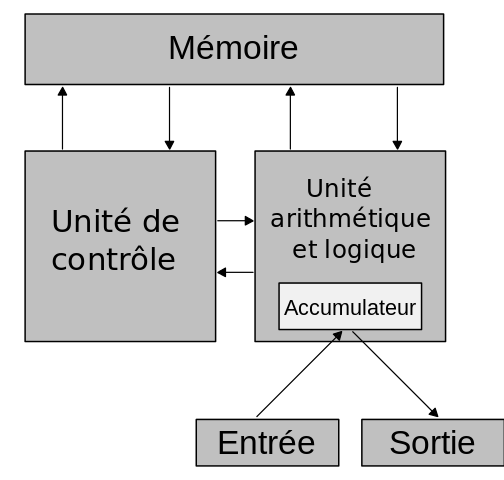
\includegraphics{Von_Neumann_architecture_fr.svg.png}
\caption{``Modèle de Von Neumann''}
\end{figure}

    \hypertarget{exercice-50}{%
\subsection{Exercice 50}\label{exercice-50}}

Parmi les quatre expressions suivantes, laquelle s'évalue en True ?

Réponses :

\begin{enumerate}
\def\labelenumi{\arabic{enumi}.}
\item
  \textbf{Réponse 1 :} \texttt{False\ and\ (True\ and\ False)}
\item
  \textbf{Réponse 2 :} \texttt{False\ or\ (True\ and\ False)}
\item
  \textbf{Réponse 3 :} \texttt{True\ and\ (True\ and\ False)}
\item
  \textbf{Réponse 4 :} \texttt{True\ or\ (True\ and\ False)}
\end{enumerate}

    \textbf{Corrigé} : La réponse est la 4.

    \begin{Verbatim}[commandchars=\\\{\}]
{\color{incolor}In [{\color{incolor}17}]:} \PY{k}{for} \PY{n}{exp} \PY{o+ow}{in} \PY{p}{[}\PY{l+s+s1}{\PYZsq{}}\PY{l+s+s1}{False and (True and False)}\PY{l+s+s1}{\PYZsq{}}\PY{p}{,} \PY{l+s+s1}{\PYZsq{}}\PY{l+s+s1}{False or (True and False)}\PY{l+s+s1}{\PYZsq{}}\PY{p}{,}\PY{l+s+s1}{\PYZsq{}}\PY{l+s+s1}{True and (True and False)}\PY{l+s+s1}{\PYZsq{}}\PY{p}{,}\PY{l+s+s1}{\PYZsq{}}\PY{l+s+s1}{True or (True and False)}\PY{l+s+s1}{\PYZsq{}}\PY{p}{]}\PY{p}{:}
             \PY{n+nb}{print}\PY{p}{(}\PY{l+s+s2}{\PYZdq{}}\PY{l+s+s2}{Valeur booléenne de }\PY{l+s+s2}{\PYZdq{}}\PY{p}{,} \PY{n}{exp}\PY{p}{,} \PY{l+s+s2}{\PYZdq{}}\PY{l+s+s2}{ = }\PY{l+s+s2}{\PYZdq{}}\PY{p}{,} \PY{n+nb}{eval}\PY{p}{(}\PY{n}{exp}\PY{p}{)}\PY{p}{)}
\end{Verbatim}


    \begin{Verbatim}[commandchars=\\\{\}]
Valeur booléenne de  False and (True and False)  =  False
Valeur booléenne de  False or (True and False)  =  False
Valeur booléenne de  True and (True and False)  =  False
Valeur booléenne de  True or (True and False)  =  True

    \end{Verbatim}

    T est un tableau de nombres entiers non vide. Que représente la valeur
de s~renvoyée par cette fonction ?

\begin{Shaded}
\begin{Highlighting}[]
\KeywordTok{def}\NormalTok{ mystere(T):}
\NormalTok{    s }\OperatorTok{=} \DecValTok{0}
    \ControlFlowTok{for}\NormalTok{ k }\KeywordTok{in}\NormalTok{ T:}
        \ControlFlowTok{if}\NormalTok{ k }\OperatorTok{\%} \DecValTok{2} \OperatorTok{==} \DecValTok{0}\NormalTok{:}
\NormalTok{            s }\OperatorTok{=}\NormalTok{ s}\OperatorTok{+}\NormalTok{k}
    \ControlFlowTok{return}\NormalTok{ s}
\end{Highlighting}
\end{Shaded}

Réponses :

\begin{enumerate}
\def\labelenumi{\arabic{enumi}.}
\item
  \textbf{Réponse 1 :} la somme des valeurs du tableau T
\item
  \textbf{Réponse 2 :} la somme des valeurs positives du tableau T
\item
  \textbf{Réponse 3 :} la somme des valeurs impaires du tableau T
\item
  \textbf{Réponse 4 :} la somme des valeurs paires du tableau T
\end{enumerate}

    \textbf{Corrigé} : La réponse est la 4.

    \begin{Verbatim}[commandchars=\\\{\}]
{\color{incolor}In [{\color{incolor}21}]:} \PY{k}{def} \PY{n+nf}{mystere}\PY{p}{(}\PY{n}{T}\PY{p}{)}\PY{p}{:}
             \PY{n}{s} \PY{o}{=} \PY{l+m+mi}{0}
             \PY{k}{for} \PY{n}{k} \PY{o+ow}{in} \PY{n}{T}\PY{p}{:}
                 \PY{k}{if} \PY{n}{k} \PY{o}{\PYZpc{}} \PY{l+m+mi}{2} \PY{o}{==} \PY{l+m+mi}{0}\PY{p}{:}
                     \PY{n}{s} \PY{o}{=} \PY{n}{s}\PY{o}{+}\PY{n}{k}
             \PY{k}{return} \PY{n}{s}
         
         \PY{k}{assert} \PY{n}{mystere}\PY{p}{(}\PY{p}{[}\PY{l+m+mi}{1}\PY{p}{,} \PY{l+m+mi}{2}\PY{p}{,} \PY{l+m+mi}{5}\PY{p}{,} \PY{l+m+mi}{4}\PY{p}{]}\PY{p}{)} \PY{o}{==} \PY{l+m+mi}{6}\PY{p}{,} \PY{l+s+s2}{\PYZdq{}}\PY{l+s+s2}{mystere([1, 2,5, 4]) doit être égal à 6}\PY{l+s+s2}{\PYZdq{}}
\end{Verbatim}


    \hypertarget{exercice-51}{%
\subsection{Exercice 51}\label{exercice-51}}

Sachant que l'expression \texttt{not(a\ or\ b)} a la valeur
\texttt{True}, quelles peuvent être les valeurs des variables booléennes
a et b~?

Réponses :

\begin{enumerate}
\def\labelenumi{\arabic{enumi}.}
\tightlist
\item
  \texttt{True} et \texttt{True}
\item
  \texttt{False} et \texttt{True}
\item
  \texttt{True} et \texttt{False}
\item
  \texttt{False} et \texttt{False}
\end{enumerate}

    \textbf{Corrigé} : La réponse est la 4. Si \texttt{not(a\ or\ b)} a la
valeur \texttt{True} alors \texttt{a\ or\ b} a la valeur \texttt{False}
et ceci n'est possible que si \texttt{a} et \texttt{b} ont la valeur
\texttt{False}.

    \hypertarget{exercice-52}{%
\subsection{Exercice 52}\label{exercice-52}}

A quelle expression logique correspond cette table de vérité ?

\begin{longtable}[]{@{}cll@{}}
\toprule
A & B & f(A, B)\tabularnewline
\midrule
\endhead
0 & 0 & 1\tabularnewline
0 & 1 & 1\tabularnewline
1 & 0 & 1\tabularnewline
1 & 1 & 0\tabularnewline
\bottomrule
\end{longtable}

    \textbf{Corrigé} : f(A, B) = NON(A ET B)

    \hypertarget{exercice-53}{%
\subsection{Exercice 53}\label{exercice-53}}

A quelle expression logique correspond cette table de vérité ?

\begin{longtable}[]{@{}cll@{}}
\toprule
A & B & f(A, B)\tabularnewline
\midrule
\endhead
0 & 0 & 0\tabularnewline
0 & 1 & 0\tabularnewline
1 & 0 & 0\tabularnewline
1 & 1 & 1\tabularnewline
\bottomrule
\end{longtable}

    \textbf{Corrigé} : f(A, B) = A ET B

    \hypertarget{exercice-54}{%
\subsection{Exercice 54}\label{exercice-54}}

A quelle expression logique correspond cette table de vérité ?

\begin{longtable}[]{@{}cll@{}}
\toprule
A & B & f(A, B)\tabularnewline
\midrule
\endhead
0 & 0 & 0\tabularnewline
0 & 1 & 1\tabularnewline
1 & 0 & 1\tabularnewline
1 & 1 & 1\tabularnewline
\bottomrule
\end{longtable}

    \textbf{Corrigé} : f(A, B) = A OU B

    \hypertarget{exercice-55}{%
\subsection{Exercice 55}\label{exercice-55}}

A quelle expression logique correspond cette table de vérité ?

\begin{longtable}[]{@{}cll@{}}
\toprule
A & B & f(A, B)\tabularnewline
\midrule
\endhead
0 & 0 & 0\tabularnewline
0 & 1 & 1\tabularnewline
1 & 0 & 1\tabularnewline
1 & 1 & 0\tabularnewline
\bottomrule
\end{longtable}

    \textbf{Corrigé} : f(A, B) = (NON(A) ET B) OU (A ET NON(B))

    \hypertarget{exercice-56}{%
\subsection{Exercice 56}\label{exercice-56}}

Choisir une expression booléenne pour la variable S qui satisfait la
table de vérité suivante.

\begin{longtable}[]{@{}lll@{}}
\toprule
A & B & S\tabularnewline
\midrule
\endhead
0 & 0 & 1\tabularnewline
0 & 1 & 0\tabularnewline
1 & 0 & 1\tabularnewline
1 & 1 & 1\tabularnewline
\bottomrule
\end{longtable}

Réponse :

\begin{enumerate}
\def\labelenumi{\arabic{enumi}.}
\tightlist
\item
  A ou (non B)
\item
  (non A) ou B
\item
  (non A) ou (non B)
\item
  non (A ou B)
\end{enumerate}

    \textbf{Corrigé} : f(A, B) = (NON(A) ET B) OU (A ET NON(B))

    \hypertarget{exercice-57} \DecValTok{2} \OperatorTok{==} \DecValTok{0}\NormalTok{:}
\NormalTok{            s }\OperatorTok{=}\NormalTok{ s}\OperatorTok{+}\NormalTok{k}
    \ControlFlowTok{return}\NormalTok{ s}
\end{Highlighting}
\end{Shaded}

Réponses :

\begin{enumerate}
\def\labelenumi{\arabic{enumi}.}
\item
  \textbf{Réponse 1 :} la somme des valeurs du tableau T
\item
  \textbf{Réponse 2 :} la somme des valeurs positives du tableau T
\item
  \textbf{Réponse 3 :} la somme des valeurs impaires du tableau T
\item
  \textbf{Réponse 4 :} la somme des valeurs paires du tableau T
\end{enumerate}

    \textbf{Corrigé} : Réponse 4

    \begin{Verbatim}[commandchars=\\\{\}]
{\color{incolor}In [{\color{incolor}68}]:} \PY{k}{def} \PY{n+nf}{mystere}\PY{p}{(}\PY{n}{T}\PY{p}{)}\PY{p}{:}
             \PY{n}{s} \PY{o}{=} \PY{l+m+mi}{0}
             \PY{k}{for} \PY{n}{k} \PY{o+ow}{in} \PY{n}{T}\PY{p}{:}
                 \PY{k}{if} \PY{n}{k} \PY{o}{\PYZpc{}} \PY{l+m+mi}{2} \PY{o}{==} \PY{l+m+mi}{0}\PY{p}{:}
                     \PY{n}{s} \PY{o}{=} \PY{n}{s}\PY{o}{+}\PY{n}{k}
             \PY{k}{return} \PY{n}{s}
\end{Verbatim}


    \begin{Verbatim}[commandchars=\\\{\}]
{\color{incolor}In [{\color{incolor}69}]:} \PY{n}{mystere}\PY{p}{(}\PY{p}{[}\PY{l+m+mi}{0}\PY{p}{,}\PY{l+m+mi}{1}\PY{p}{,}\PY{l+m+mi}{2}\PY{p}{,}\PY{l+m+mi}{3}\PY{p}{,}\PY{l+m+mi}{4}\PY{p}{]}\PY{p}{)}
\end{Verbatim}


\begin{Verbatim}[commandchars=\\\{\}]
{\color{outcolor}Out[{\color{outcolor}69}]:} 6
\end{Verbatim}
            
    \hypertarget{exercice-58}{%
\subsection{Exercice 58}\label{exercice-58}}

Soit \(n\) un entier naturel. Sa factorielle est le produit des nombres
entiers strictement positifs qui sont plus petits ou égaux à \(n\). Par
exemple la factorielle de 4 vaut \(1 \times 2 \times 3 \times 4 = 24\).

Quelle est la fonction correcte parmi les suivantes ?

Réponses :

\begin{enumerate}
\def\labelenumi{\arabic{enumi}.}
\item
  \textbf{Réponse 1 :} \textasciitilde{}\sout{python def factorielle(n):
  i = 0 fact = 1 while i \textless= n: fact = fact * i i = i + 1 return
  fact}\textasciitilde{}
\item
  \textbf{Réponse 2 :} \textasciitilde{}\sout{python def factorielle(n):
  i = 1 fact = 1 while i \textless{} n: fact = fact * i i = i + 1 return
  fact}\textasciitilde{}
\item
  \textbf{Réponse 3 :}\\
  \textasciitilde{}\sout{python def factorielle(n): i = 0 fact = 1 while
  i \textless{} n: i = i + 1 fact = fact * i return
  fact}\textasciitilde{}
\item
  \textbf{Réponse 4 :} \textasciitilde{}\sout{python def factorielle(n):
  i = 0 fact = 1 while i \textless= n: i = i + 1 fact = fact * i return
  fact}\textasciitilde{}
\end{enumerate}

    \textbf{Corrigé} : Réponse 3

    \begin{Verbatim}[commandchars=\\\{\}]
{\color{incolor}In [{\color{incolor}71}]:} \PY{k+kn}{from} \PY{n+nn}{math} \PY{k}{import} \PY{n}{factorial}
         
         \PY{k}{def} \PY{n+nf}{factorielle}\PY{p}{(}\PY{n}{n}\PY{p}{)}\PY{p}{:}
              \PY{n}{i} \PY{o}{=} \PY{l+m+mi}{0}
              \PY{n}{fact} \PY{o}{=} \PY{l+m+mi}{1}
              \PY{k}{while} \PY{n}{i} \PY{o}{\PYZlt{}} \PY{n}{n}\PY{p}{:}
                  \PY{n}{i} \PY{o}{=} \PY{n}{i} \PY{o}{+} \PY{l+m+mi}{1}
                  \PY{n}{fact} \PY{o}{=} \PY{n}{fact} \PY{o}{*} \PY{n}{i}
              \PY{k}{return} \PY{n}{fact}
         
         \PY{p}{[}\PY{n}{factorial}\PY{p}{(}\PY{n}{n}\PY{p}{)} \PY{o}{==} \PY{n}{factorielle}\PY{p}{(}\PY{n}{n}\PY{p}{)} \PY{k}{for} \PY{n}{n} \PY{o+ow}{in} \PY{n+nb}{range}\PY{p}{(}\PY{l+m+mi}{0}\PY{p}{,} \PY{l+m+mi}{10}\PY{p}{)}\PY{p}{]}
\end{Verbatim}


\begin{Verbatim}[commandchars=\\\{\}]
{\color{outcolor}Out[{\color{outcolor}71}]:} [True, True, True, True, True, True, True, True, True, True]
\end{Verbatim}
            
    \hypertarget{exercice-59}{%
\subsection{Exercice 59}\label{exercice-59}}

Écrire une fonction \texttt{min2(a,\ b)} qui retourne le minimum de deux
nombres passés en paramètre, sans utiliser la fonction \texttt{min} du
module \texttt{builtins}.

    \textbf{Corrigé} : Ci-dessous

    \begin{Verbatim}[commandchars=\\\{\}]
{\color{incolor}In [{\color{incolor}72}]:} \PY{k}{def} \PY{n+nf}{min2}\PY{p}{(}\PY{n}{a}\PY{p}{,} \PY{n}{b}\PY{p}{)}\PY{p}{:}
             \PY{k}{if} \PY{n}{a} \PY{o}{\PYZlt{}} \PY{n}{b}\PY{p}{:}
                 \PY{k}{return} \PY{n}{a}
             \PY{k}{else}\PY{p}{:}
                 \PY{k}{return} \PY{n}{b}
\end{Verbatim}


    \hypertarget{exercice-60}{%
\subsection{Exercice 60}\label{exercice-60}}

En voulant programmer une fonction qui calcule la valeur minimale d'une
liste d'entiers, on a écrit :

\begin{Shaded}
\begin{Highlighting}[]
\KeywordTok{def}\NormalTok{ minimum(L):}
\NormalTok{    mini }\OperatorTok{=} \DecValTok{0}
    \ControlFlowTok{for}\NormalTok{ e }\KeywordTok{in}\NormalTok{ L:}
        \ControlFlowTok{if}\NormalTok{ e }\OperatorTok{<}\NormalTok{ mini:}
\NormalTok{            mini }\OperatorTok{=}\NormalTok{ e}
    \ControlFlowTok{return}\NormalTok{ mini}
\end{Highlighting}
\end{Shaded}

Cette fonction a été mal programmée. Pour quelle liste ne donnera-t-elle
pas le résultat attendu, c'est-à-dire son minimum ?

Réponses :

\begin{enumerate}
\def\labelenumi{\arabic{enumi}.}
\tightlist
\item
  \textbf{Réponse 1 :} \texttt{{[}-1,-8,12,2,23{]}}
\item
  \textbf{Réponse 2:} \texttt{{[}0,18,12,2,3{]}}
\item
  \textbf{Réponse 3:} \texttt{{[}-1,-1,12,12,23{]}}
\item
  \textbf{Réponse 4:} \texttt{{[}1,8,12,2,23{]}}
\end{enumerate}

    \textbf{Corrigé} : Pour une liste d'éléments tous strictement positifs,
comme celle de la réponse 4, la fonction retournera 0. Il aurait fallu
initialiser \texttt{mini} avec \texttt{L{[}0{]}}.

    \hypertarget{exercice-61}{%
\subsection{Exercice 61}\label{exercice-61}}

Écrire une fonction \texttt{min\_liste(L)} qui retourne le minimum d'une
liste de nombres passée en paramètre.

    \textbf{Corrigé} : voir ci-dessous.

    \begin{Verbatim}[commandchars=\\\{\}]
{\color{incolor}In [{\color{incolor}73}]:} \PY{k}{def} \PY{n+nf}{min\PYZus{}liste}\PY{p}{(}\PY{n}{L}\PY{p}{)}\PY{p}{:}
             \PY{n}{mini} \PY{o}{=} \PY{n}{L}\PY{p}{[}\PY{l+m+mi}{0}\PY{p}{]}
             \PY{k}{for} \PY{n}{k} \PY{o+ow}{in} \PY{n+nb}{range}\PY{p}{(}\PY{l+m+mi}{1}\PY{p}{,} \PY{n+nb}{len}\PY{p}{(}\PY{n}{L}\PY{p}{)}\PY{p}{)}\PY{p}{:}
                 \PY{k}{if} \PY{n}{L}\PY{p}{[}\PY{n}{k}\PY{p}{]} \PY{o}{\PYZlt{}} \PY{n}{mini} \PY{p}{:}
                     \PY{n}{mini} \PY{o}{=} \PY{n}{L}\PY{p}{[}\PY{n}{k}\PY{p}{]}
             \PY{k}{return} \PY{n}{mini}  
\end{Verbatim}


    \hypertarget{exercice-62}{%
\subsection{Exercice 62}\label{exercice-62}}

Quelle est la valeur de element à la fin de l'exécution du code suivant
:

\begin{Shaded}
\begin{Highlighting}[]
\NormalTok{L }\OperatorTok{=}\NormalTok{ [}\DecValTok{1}\NormalTok{,}\DecValTok{2}\NormalTok{,}\DecValTok{3}\NormalTok{,}\DecValTok{4}\NormalTok{,}\DecValTok{1}\NormalTok{,}\DecValTok{2}\NormalTok{,}\DecValTok{3}\NormalTok{,}\DecValTok{4}\NormalTok{,}\DecValTok{0}\NormalTok{,}\DecValTok{2}\NormalTok{]}
\NormalTok{element }\OperatorTok{=}\NormalTok{ L[}\DecValTok{0}\NormalTok{]}
\ControlFlowTok{for}\NormalTok{ k }\KeywordTok{in}\NormalTok{ L:}
    \ControlFlowTok{if}\NormalTok{ k }\OperatorTok{>}\NormalTok{ element:}
\NormalTok{        element }\OperatorTok{=}\NormalTok{ k}
\end{Highlighting}
\end{Shaded}

\begin{enumerate}
\def\labelenumi{\arabic{enumi}.}
\tightlist
\item
  \textbf{Réponse 1 :} 0
\item
  \textbf{Réponse 2:} 1
\item
  \textbf{Réponse 3:} 4
\item
  \textbf{Réponse 4:} 10
\end{enumerate}

    \textbf{Corrigé} : la réponse est 4, le maximum de la liste \texttt{L}.

    \hypertarget{exercice-63}{%
\subsection{Exercice 63}\label{exercice-63}}

Un élève a écrit la fonction ci-dessus pour déterminer si le premier
paramètre n est dans la liste L passée en second paramètre. Le
professeur lui indique que son code comporte des erreurs. Proposer une
version corrigée de cette fonction.

\begin{Shaded}
\begin{Highlighting}[]
\KeywordTok{def}\NormalTok{ element\_dans\_liste(n, L):}
    \ControlFlowTok{for}\NormalTok{ k }\KeywordTok{in} \BuiltInTok{range}\NormalTok{(}\BuiltInTok{len}\NormalTok{(L)):}
        \ControlFlowTok{if}\NormalTok{ e }\OperatorTok{==}\NormalTok{ n:}
            \ControlFlowTok{return} \VariableTok{True}
        \ControlFlowTok{else}\NormalTok{:}
            \ControlFlowTok{return} \VariableTok{False}
\end{Highlighting}
\end{Shaded}

    \textbf{Corrigé} : voir ci-dessous.

    \begin{Verbatim}[commandchars=\\\{\}]
{\color{incolor}In [{\color{incolor} }]:} \PY{k}{def} \PY{n+nf}{element\PYZus{}dans\PYZus{}liste}\PY{p}{(}\PY{n}{n}\PY{p}{,} \PY{n}{L}\PY{p}{)}\PY{p}{:}
            \PY{k}{for} \PY{n}{k} \PY{o+ow}{in} \PY{n+nb}{range}\PY{p}{(}\PY{n+nb}{len}\PY{p}{(}\PY{n}{L}\PY{p}{)}\PY{p}{)}\PY{p}{:}
                \PY{k}{if} \PY{n}{e} \PY{o}{==} \PY{n}{n}\PY{p}{:}
                    \PY{k}{return} \PY{k+kc}{True}
                \PY{k}{else}\PY{p}{:}
                    \PY{k}{return} \PY{k+kc}{False}
\end{Verbatim}


    \hypertarget{exercice-64}{%
\subsection{Exercice 64}\label{exercice-64}}

Pour chacune des listes ci-dessous, déterminer si l'algorithme le plus
adapté pour qu'une machine y recherche une valeur est l'algorithme de
recherche séquentielle ou l'algorithme de recherche dichotomique.

\begin{enumerate}
\def\labelenumi{\arabic{enumi}.}
\tightlist
\item
  Liste A :
  \texttt{{[}4,\ 6,\ 15,\ 20,\ 21,\ 26,\ 31,\ 41,\ 42,\ 50,\ 69,\ 87,\ 88,\ 92,\ 97{]}}
\item
  Liste B :
  \texttt{{[}41,\ 97,\ 91,\ 59,\ 7,\ 45,\ 3,\ 96,\ 26,\ 32,\ 18,\ 11,\ 67,\ 74,\ 54{]}}
\end{enumerate}

    \textbf{Corrigé} :

\begin{itemize}
\tightlist
\item
  La liste A est triée dans l'ordre croissant donc on peut lui appliquer
  une recherche dichotomique qui est plus efficace que la recherche
  séquentielle
\item
  la liste B n'est pas ordonnée donc on ne peut pas lui appliquer une
  recherche dichotomique mais uniquement une recherche séquentielle
\end{itemize}

    \hypertarget{exercice-65}{%
\subsection{Exercice 65}\label{exercice-65}}

Compléter le code de la fonction \texttt{recherche\_dicho\_dec(x,\ L)}
qui prend en paramètres un nombre \texttt{x} et une liste de nombres
\texttt{L} triée dans l'ordre décroissant. Elle doit retourner
\texttt{True} si \texttt{x} appartient à L et False sinon.

\begin{Shaded}
\begin{Highlighting}[]
\KeywordTok{def}\NormalTok{ recherche\_dicho\_dec(x, L):}
\NormalTok{    a, b }\OperatorTok{=} \DecValTok{0}\NormalTok{, }\BuiltInTok{len}\NormalTok{(L) }\OperatorTok{{-}} \DecValTok{1}
    \ControlFlowTok{while}\NormalTok{ a }\OperatorTok{<=}\NormalTok{ b:}
\NormalTok{        m }\OperatorTok{=}\NormalTok{ (a }\OperatorTok{+}\NormalTok{ b) }\OperatorTok{//} \DecValTok{2}
        \ControlFlowTok{if}\NormalTok{ L[m] }\OperatorTok{>}\NormalTok{ x:}
\NormalTok{            ..................}
        \ControlFlowTok{elif}\NormalTok{ L[m] }\OperatorTok{<}\NormalTok{ x:}
\NormalTok{            ................}
        \ControlFlowTok{else}\NormalTok{:}
\NormalTok{            .................}
\NormalTok{    .........................}
\end{Highlighting}
\end{Shaded}

    \textbf{Corrigé} : voir ci-dessous

    \begin{Verbatim}[commandchars=\\\{\}]
{\color{incolor}In [{\color{incolor}74}]:} \PY{k}{def} \PY{n+nf}{recherche\PYZus{}dicho\PYZus{}dec}\PY{p}{(}\PY{n}{x}\PY{p}{,} \PY{n}{L}\PY{p}{)}\PY{p}{:}
             \PY{n}{a}\PY{p}{,} \PY{n}{b} \PY{o}{=} \PY{l+m+mi}{0}\PY{p}{,} \PY{n+nb}{len}\PY{p}{(}\PY{n}{L}\PY{p}{)} \PY{o}{\PYZhy{}} \PY{l+m+mi}{1}
             \PY{k}{while} \PY{n}{a} \PY{o}{\PYZlt{}}\PY{o}{=} \PY{n}{b}\PY{p}{:}
                 \PY{n}{m} \PY{o}{=} \PY{p}{(}\PY{n}{a} \PY{o}{+} \PY{n}{b}\PY{p}{)} \PY{o}{/}\PY{o}{/} \PY{l+m+mi}{2}
                 \PY{k}{if} \PY{n}{L}\PY{p}{[}\PY{n}{m}\PY{p}{]} \PY{o}{\PYZgt{}} \PY{n}{x}\PY{p}{:}
                     \PY{n}{b} \PY{o}{=} \PY{n}{m} \PY{o}{\PYZhy{}} \PY{l+m+mi}{1}
                 \PY{k}{elif} \PY{n}{L}\PY{p}{[}\PY{n}{m}\PY{p}{]} \PY{o}{\PYZlt{}} \PY{n}{x}\PY{p}{:}
                     \PY{n}{a} \PY{o}{=} \PY{n}{m} \PY{o}{+} \PY{l+m+mi}{1}
                 \PY{k}{else}\PY{p}{:}
                     \PY{k}{return} \PY{k+kc}{True}
             \PY{k}{return} \PY{k+kc}{False}
\end{Verbatim}


    \hypertarget{exercice-66}{%
\subsection{Exercice 66}\label{exercice-66}}

\emph{Auteur Sylvie Genre}

La fonction suivante doit calculer la moyenne d'un tableau de nombres,
passé en paramètre. Avec quelles expressions faut-il remplacer les
points de suspension pour que la fonction soit correcte ?

\begin{Shaded}
\begin{Highlighting}[]
\KeywordTok{def}\NormalTok{ moyenne(tableau):}
\NormalTok{    total }\OperatorTok{=}\NormalTok{ ...}
    \ControlFlowTok{for}\NormalTok{ valeur }\KeywordTok{in}\NormalTok{ tableau:}
\NormalTok{        total }\OperatorTok{=}\NormalTok{ total }\OperatorTok{+}\NormalTok{ valeur}
    \ControlFlowTok{return}\NormalTok{ total }\OperatorTok{/}\NormalTok{ ...}
\end{Highlighting}
\end{Shaded}

Réponses :

\begin{enumerate}
\def\labelenumi{\arabic{enumi}.}
\tightlist
\item
  \textbf{Réponse 1 :} 1 et \texttt{(len(tableau)\ +\ 1)}
\item
  \textbf{Réponse 2:} 0 et \texttt{(len(tableau)\ +\ 1)}
\item
  \textbf{Réponse 3:} 0 et \texttt{len(tableau)}
\end{enumerate}

    \textbf{Corrigé} : Réponse 3

    \hypertarget{exercice-67}{%
\subsection{Exercice 67}\label{exercice-67}}

On considère le code incomplet suivant qui recherche le maximum dans une
liste.

\begin{Shaded}
\begin{Highlighting}[]
\NormalTok{liste }\OperatorTok{=}\NormalTok{ [}\DecValTok{5}\NormalTok{,}\DecValTok{12}\NormalTok{,}\DecValTok{15}\NormalTok{,}\DecValTok{3}\NormalTok{,}\DecValTok{15}\NormalTok{,}\DecValTok{17}\NormalTok{,}\DecValTok{29}\NormalTok{,}\DecValTok{1}\NormalTok{]}
\NormalTok{iMax }\OperatorTok{=} \DecValTok{0}
\ControlFlowTok{for}\NormalTok{ i }\KeywordTok{in} \BuiltInTok{range}\NormalTok{(}\DecValTok{1}\NormalTok{,}\BuiltInTok{len}\NormalTok{(liste)):}
\NormalTok{    .........}
\NormalTok{iMax }\OperatorTok{=}\NormalTok{ i}
\BuiltInTok{print}\NormalTok{ (liste[iMax])}
\end{Highlighting}
\end{Shaded}

Par quoi faut-il remplacer la ligne pointillée ?

Réponses :

\begin{enumerate}
\def\labelenumi{\arabic{enumi}.}
\tightlist
\item
  \textbf{Réponse 1 :} \texttt{if\ i\ \textgreater{}\ iMax:}
\item
  \textbf{Réponse 2:}
  \texttt{if\ liste{[}i{]}\ \textgreater{}\ liste{[}iMax{]}:}
\item
  \textbf{Réponse 3:} \texttt{if\ liste{[}i{]}\ \textgreater{}\ iMax:}
\item
  \textbf{Réponse 4:} \texttt{if\ i\ \textgreater{}\ liste{[}iMax{]}:}
\end{enumerate}

    \textbf{Corrigé} : Réponse 32

    \hypertarget{exercice-68}{%
\subsection{Exercice 68}\label{exercice-68}}

Le protocole qui permet à un client de faire une requête de page Web
auprès d'un serveur Web s'appelle :

Réponses :

\begin{enumerate}
\def\labelenumi{\arabic{enumi}.}
\tightlist
\item
  Internet Protocol
\item
  HTML
\item
  HTTP
\item
  SMTP
\item
  WWW
\end{enumerate}

    \textbf{Corrigé} : Réponse 3 HTTP pour Hypertext Transfer Protocol

    \hypertarget{exercice-69}{%
\subsection{Exercice 69}\label{exercice-69}}

Si la page demandée n'est pas disponible, le serveur Web renvoie au
client un code d'erreur :

Réponses :

\begin{enumerate}
\def\labelenumi{\arabic{enumi}.}
\item
  404
\item
  504
\item
  403
\item
  503
\end{enumerate}

    \textbf{Corrigé} : Réponse 1 Erreur 404

    \hypertarget{exercice-70}{%
\subsection{Exercice 70}\label{exercice-70}}

L'inventeur du World Wide Web au CERN est :

Réponses :

\begin{enumerate}
\def\labelenumi{\arabic{enumi}.}
\item
  Tim Berners-Lee
\item
  Ted Nelson
\item
  Louis Pouzin
\item
  Vinton Cerf
\end{enumerate}

    \textbf{Corrigé} : Réponse 1 Tim Berners-Lee

    \hypertarget{exercice-71}{%
\subsection{Exercice 71}\label{exercice-71}}

Dans le fichier source d'une page Web, le code qui permet de créer un
lien hypertexte vers la page \url{https://www.w3schools.com/} est :

Réponses :

\begin{enumerate}
\def\labelenumi{\arabic{enumi}.}
\item
  \texttt{\textless{}a\ href="https://www.w3schools.com/"\textgreater{}https://www.w3schools.com/\textless{}/a\textgreater{}}
\item
  \texttt{\textless{}a\ href="lien\ hypertexte"\textgreater{}https://www.w3schools.com/\textless{}/a\textgreater{}}
\item
  \texttt{\textless{}a\ href="https://www.w3schools.com/"\textgreater{}lien\ hypertexte\textless{}/a\textgreater{}}
\item
  \texttt{\textless{}href\ a="https://www.w3schools.com/"\textgreater{}lien\ hypertexte\textless{}/href\textgreater{}}
\end{enumerate}

    \textbf{Corrigé} : Réponse 3

    \hypertarget{exercice-72}{%
\subsection{Exercice 72}\label{exercice-72}}

Pour créer un lien vers la page d'accueil de Wikipédia, que devra-t-on
écrire dans une page Web ?

\textbf{Réponses :}

\begin{enumerate}
\def\labelenumi{\arabic{enumi}.}
\item
  \textbf{Réponse 1 :}
  \texttt{\textless{}a\ target="http://fr.wikipedia.org"\textgreater{}Wikipédia\textless{}/a\textgreater{}}
\item
  \textbf{Réponse 2 :}
  \texttt{\textless{}a\ href="http://fr.wikipedia.org"\textgreater{}}
\item
  \textbf{Réponse 3 :}
  \texttt{\textless{}a\ href="http://fr.wikipedia.org"\textgreater{}Wikipédia\textless{}/a\textgreater{}}
\item
  \textbf{Réponse 4 :}
  \texttt{\textless{}link\ src="http://fr.wikipedia.org"\textgreater{}Wikipédia\textless{}/link\textgreater{}}
\end{enumerate}

    \textbf{Corrigé} : Réponse 3


    % Add a bibliography block to the postdoc
    
    
    
    \end{document}
